\documentclass[12pt]{report}
\renewcommand{\baselinestretch}{1}
\usepackage{braket}
\usepackage{wrapfig}
\usepackage{dsfont}
\usepackage[utf8]{inputenc}
\usepackage{amsmath}
\usepackage{graphicx}
\usepackage{subcaption}
\usepackage[left=2.5cm,top=2cm,right=2.5cm,bottom=2.5cm]{geometry}
\usepackage{multicol}
\usepackage{authblk}
\usepackage{subcaption}
\usepackage{cite}
\usepackage{mwe}
\usepackage[font={small,it}]{caption}
\graphicspath{{./img/}}


%user-defined commands

\newcommand{\qty}[1]
{
	\left({#1}\right)
}


\font\myfont=cmr12 at 16pt


\title{\bf{Mathematical model for the concentration and electric potential profiles in a solution of electrolytes under a redox reaction}}

\author{{\myfont Student: Agust\'in Escobar Blanc\\Professor: Enrique Mu\~ noz Tavera}}
\affil{\textit{Departamento de F\'isica, Facultad de F\'isica, Pontificia Universidad Cat\'olica de Chile}}

\begin{document}

\maketitle

\tableofcontents

\chapter{Diffusion Of Electrolytes In Solution}
\section{Diffusion Of Electrolytes In Electro-refining Context}

We know that electro-refining  apperas to be
\begin{eqnarray}
\frac{\partial C_+}{\partial t}+\nabla\cdot \mathbf{N}_+ = 0, \\
\frac{\partial C_-}{\partial t}+\nabla\cdot \mathbf{N}_- = 0, \\
\nabla^2\phi(x)=-\frac{\rho(x)}{\epsilon}.
\end{eqnarray}
Where $C_s$ is the concentration of each species and $N_s$ is the diffusive flux for each species.
In our model, the flux is defined as

$$\mathbf{N}_+= -D_+\left(\nabla C_+(x) +\frac{z_+ F}{RT}C_+(x)\nabla\phi(x)\right)$$,
$$\mathbf{N}_-= -D_-\left(\nabla C_-(x) +\frac{z_- F}{RT}C_-(x)\nabla\phi(x)\right)$$.

Therefore, the diffusion equation with electric field interaction incorporated is \cite{Dolde2011}

\begin{eqnarray}
\frac{\partial C_+}{\partial t}=\nabla\cdot\left[ \mathcal{D}_+\left(\nabla C_+(x) +\frac{z F}{RT}C_+(x)\nabla\phi(x)\right)\right]= 0, \\
\frac{\partial C_-}{\partial t}=\nabla\cdot\left[ \mathcal{D}_-\left(\nabla C_-(x) -\frac{z F}{RT}C_-(x)\nabla\phi(x)\right)\right] = 0.
\end{eqnarray}

where $z = |z_+|=|z_-|$ is the valence of the electrolyte, $D_{\pm}$ are the diffusion coefficients for each chemical species and $F = 96485.33\,C\,mol^{-1}$ is Faraday's constant.

The reaction we are modeling is the cation reduction. In particular, we are interested in copper reduction at the surface
\begin{equation}
Cu^{+2} + 2 e^{-} \rightarrow Cu^{0}.
\end{equation}

This chemical reaction yields the following border condition for the flux
\begin{eqnarray}
\left.\mathbf{N}_{+}\cdot\hat{n}\right|_{Surface} &=& \frac{I_{0}}{z_{+}FA},\nonumber\\
\left.\mathbf{N}_{-}\cdot\hat{n}\right|_{Surface} &=& 0.
\label{eq_bc1}
\end{eqnarray}

with $A$ being the total area of the surface, $I_{0}$ the total electric current and $\hat{n}$ the unit normal of the surface.


\chapter{Steady State Solution}
\section{Linearization of the Poisson Equation}

As a first approach to solving the equilibrium system (that is, system when there is no current at all), we can simplify the Poisson-Boltzmann Equation by linearizing the Boltzmann term in the Debye-Huckle theory to first order in the potential
The Poisson-Boltzmann equation is

$$-\frac{d^2\phi(x)}{dx^2}  =\frac{1}{\epsilon}\sum_s z_s F C_{b,s} e^{\frac{z_s F \phi(x)}{RT}},$$
which by expanding the exponential for $\left|\frac{z_s F \phi(x)}{RT}\right| < 1$ we get
$$-\frac{d^2\phi(x)}{dx^2} =\frac{1}{\epsilon}\sum_s z_s F C_s \left(1-\frac{z_s F \phi(x)}{RT}\right)$$

Due to electro-neutrality in the bulk solution, the first term in the right hand side is zero. Therefore, 
$$\frac{d^2\phi(x)}{dx^2} =\kappa^2 \phi(x)$$

where we have defined 
$$\kappa = \sqrt{\frac{\sum_s C_{b,s} z_s^2 F^2}{\epsilon RT}}$$

Given the boundary conditions $\phi(0) = V_0$, and considering the reference zero at $\phi(\delta) = \phi_b = 0$, the solution is trivially found to be

$$\phi(x) = V_0 e^{-\kappa x},$$

This gives the potential in a static situation, in which the electrolytes move to an equilibrium position and the configuration as a hole is static. 

\begin{figure}[h!]
\label{fig:comparison}
 \centering
 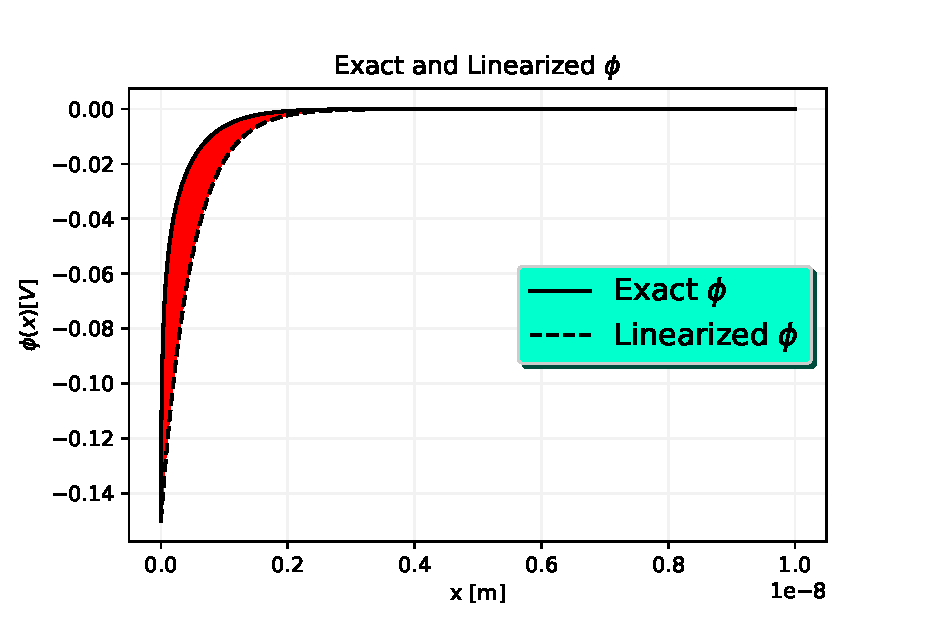
\includegraphics[width = 0.6\linewidth]{comparison-phi.eps}
 \caption{Comparison of the linearized PB solution with the analytical solution. The region in red is the error committed in this approximation}
\end{figure}

This results gives a good physical sense of how the potential should look like in a context of electrolyte solutions at equilibrium. We are interested in the dynamics of the system, though, so it makes sense to try to incorporate the current into Eq. \ref{eq:system}. In the next section we shall incorporate the current flowing through the interface as a border condition of Eq. \ref{eq:system}.

\section{Steady State Solution To The Diffusion-Reaction Problem}

In what follows, we shall assume that the system presents concentration gradients and
potential gradients along a single dimension $x$. This is equivalent to considering the interface infinitely large. Therefore, $\mathbf{N}_{+} = \hat{x}N_{+}$ and $\mathbf{N}_{-} = \hat{x}N_{-}$. 

In the steady state solution the concentration distribution of each electrolyte throughout the system should not change in time, thus

$$\frac{\partial C_+}{\partial t} = \frac{\partial C_-}{\partial t} = 0$$

This yields the following results

$$\nabla\cdot \mathbf{N}_+ = \frac{\partial N_{+}}{\partial x}=0$$
$$\nabla \cdot \mathbf{N}_- = \frac{\partial N_{-}}{\partial x}=0$$

Therefore, we have

$$N_+ = A_1$$
$$N_- = A_2$$

where $A_1$ and $A_2$ are constants determined by border conditions. Since the anion does not interact with the interface, we get after Eq.(\ref{eq_bc1})
$N_- = 0$. On the other hand, the flux due to the cation reaction with the interface ($Cu^{+2}\rightarrow Cu^{0}$) gives the boundary condition for $N_+$,

$$N_+ = \frac{I_0}{Az_+F}$$

The complete system of equations to be solved is

$$N_-(x) = 0$$

$$N_+(x) = \frac{I_0}{Aze}$$

\begin{figure}[h!]
\centering
	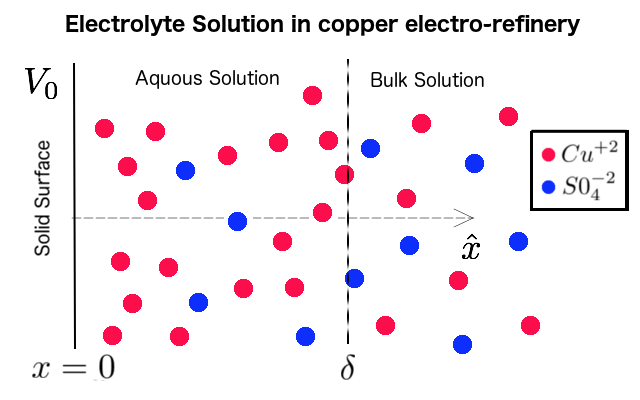
\includegraphics[width=0.5\textwidth]{geometry.png}
	\caption{Geometry of the problem. $x<\delta$ is the region of laminar. $x>\delta$ is the bulk of the solution. This image is for a value of $V_0<0$, such that the positive electrolytes distribute closer to the surface.}
\label{fig:geometry}
\end{figure}


According to Fig. \ref{fig:geometry}, for an interface area large compared to the laminar flux region we get the following equations 

\begin{eqnarray}\label{eq:system}
\frac{\partial C_+}{\partial x}-\frac{z F}{RT}C_+\frac{\partial \phi}{\partial x} &=& -\frac{I_0}{D_+Az_+ F}\label{eq:eq1} \\
\frac{\partial C_-}{\partial x}+\frac{z F}{RT}C_-\frac{\partial \phi}{\partial x} &=& 0 \label{eq:eq2}\\
\frac{\partial^2 \phi}{\partial x^2} &=& -\frac{1}{\epsilon} \sum_{s=\pm}z_s F C_s(x)\label{eq:eq3}
\end{eqnarray}

where A is the area of the interface electrode. 

To solve this system of partial differential equations, we will expand the concentration and the potential as a series in powers of $r = \frac{I_0}{D_+Az_+ F}$. We have

\begin{eqnarray}
C_s(x) = \sum_{n=0}^{\infty}r^n C_s^{(n)}(x)\\
\phi(x) = \sum_{n=0}^{\infty}r^n \phi^{(n)}(x)
\end{eqnarray}

Truncating the series at first order in $r$, we obtain the following system of equations to order zero in the current
\begin{eqnarray}
\frac{\partial C^{(0)}_+}{\partial x}-\frac{zF}{RT}C^{(0)}_+(x)\frac{\partial \phi^{(0)}}{\partial x} &=& 0\\
\label{eq:concentration-diff-zero1}
\frac{\partial C^{(0)}_-}{\partial x}+\frac{zF}{RT}C^{(0)}_-(x)\frac{\partial \phi^{(0)}}{\partial x}&=& 0\\
\label{eq:concentration-diff-zero2}
\frac{\partial^2  \phi^{(0)}}{\partial x^2} &=& -\frac{1}{\epsilon}\sum_{s= \pm} szF C^{(0)}_{s}(x)
\label{eq:concentration-diff-zero3}
\end{eqnarray}

and to first order in the current

\begin{eqnarray}
\frac{\partial C^{(1)}_+}{\partial x}-\frac{zF}{RT}\qty{C^{(1)}_+(x)\frac{\partial \phi^{(0)}}{\partial x}+C^{(0)}_+(x)\frac{\partial \phi^{(1)}}{\partial x}} &=& -1,\\
\label{eq:concentration-diff-first1}
\frac{\partial C^{(1)}_-}{\partial x}+\frac{zF}{RT}\qty{C^{(1)}_-(x)\frac{\partial \phi^{(0)}}{\partial x}+C^{(0)}_-(x)\frac{\partial \phi^{(1)}}{\partial x}}&=& 0,\\
\label{eq:concentration-diff-first2}
\frac{\partial^2  \phi^{(1)}}{\partial x^2} &=& -\frac{1}{\epsilon}\sum_{s= \pm} szF C^{(1)}_{s}(x).
\label{eq:concentration-diff-first3}
\end{eqnarray}




















\newpage

\section{Zero order solution to Poisson's equation for the electrolyte solution}
\label{sec:zeroorderphi}

We want to work with the dimensionless potential 

$$\Phi(x) = \frac{zF}{RT}\phi(x).$$

The zero order system can thus be written as

\begin{eqnarray}
\label{eq:zero-order}
C^{(0)}_+(x)'-C^{(0)}_+(x)\Phi^{(0)}(x)' &=& 0\\
 C^{(0)}_-(x)'+C^{(0)}_-(x)\Phi^{(0)}(x)'&=& 0\\
\Phi^{(0)}(x) ''&=& -\frac{(zF)^2}{RT\epsilon} (C^{(0)}_{+}(x)-C^{(0)}_{-}(x))
\end{eqnarray}



In this section we will solve equations \ref{eq:concentration-diff-first1} and \ref{eq:concentration-diff-first2}. 

From Eq. \ref{eq:zero-order},

$$\frac{\partial C^{(0)}_s}{\partial x}-sC^{(0)}_s\Phi^{(0)}(x)= 0$$

which yields

$$\int_{C_{b,s}}^{C^{(0)}_s(x)} \frac{dC^{(0)}_s}{C^{(0)}_s}=s\int_{\phi_b}^{\phi^{(0)}} d\Phi^{(0)}$$

where $\Phi_b = \Phi(\delta)$ is the potential at the bulk, which we will consider as the reference zero, $\phi_b = 0$. $C_{b,s}$ is the bulk concentration of each species in solution.

$$C^{(0)}_s(x)=C_{b,s}e^{s\Phi^{(0)}(x)}$$

Notice that 
\begin{equation}
C^{(0)}_s(\delta) = C_{b,s}e^{\frac{zF}{RT}\phi_b}=C_{b,s}.
\label{eq:zero-order-sol-c}
\end{equation}

Consider the bulk values of the concentration, $C_{s,b}$. In the bulk, the solution should be electrically neutral due to conservation of charge. Therefore, for a two electrolyte salt at the bulk

\begin{equation}
\label{eq:electroneutrality}
\sum_{s=\pm} C_{s,b} sz F = 0
\end{equation}


where $z$ is the valence of the electrolytes and $s = \pm$ is the sign of the charge of the electrolyte. $F = eN_A$ is the Faraday constant. From \ref{eq:electroneutrality} we get,

\begin{eqnarray}\nonumber
C_{b,+}Fz-C_{b,-}Fz=0\\
\rightarrow \frac{C_{b,+}}{C_{b,-}}=1
\label{eq:electroneutrality2}
\end{eqnarray}

$$C_{b,+}Fz-C_{b,-}Fz=0$$
$$\rightarrow \frac{C_{b,+}}{C_{b,-}}=1$$

In the case of a symmetric salt, $q_s=-q_{-s}$ (since in our notation $s=\pm$). Poisson's equation can be written (to zero order in the current) as

\begin{equation}
\label{eq:poisson1}
\frac{\partial^2 \Phi^{(0)}}{\partial x^2} = -\frac{zF}{\epsilon} \left(C_{b,+}e^{\Phi^{(0)}(x)}-C_{b,-}e^{-\Phi^{(0)}(x)}\right)
\end{equation}

where $z=|z_-|=|z_+|$. From equations \ref{eq:zero-order-sol-c}  and \ref{eq:electroneutrality2} we have $C_{b,+}=C_{b,+} = C_b$. Equation \ref{eq:poisson1} can be written in terms of the hyperbolic sine,

\begin{equation}
\label{eq:poisson2}
\frac{\partial^2 \Phi^{(0)}}{\partial x^2} = 2\frac{(zF)^2C_b}{RT\epsilon}\sinh{\left(\Phi^{(0)}(x)\right)}
\end{equation}

We define the quantity  

$$\kappa^2  = \frac{(zF)^2C_b}{RT\epsilon}$$

\begin{equation}
\frac{\partial^2 \Phi^{(0)}}{\partial x^2} = 2\kappa \sinh{\left(\Phi^{(0)}(x)\right)}
\end{equation}

We want to change variables to the dimensionless quantity $\kappa x$,

$$x \rightarrow \xi = \kappa x$$
 $$d \xi  = \kappa d x $$
 
Thus, we write,

\begin{equation}
\Phi^{(0)}(\xi)''= 2\sinh{\left(\Phi^{(0)}(\xi)\right)}
\end{equation}

Multiplying by  $\Phi'^{(0)}$ and integrating the equation over the interval $[\xi, \delta]$ we get,
 
\begin{align}
\Phi^{(0)}(\kappa \delta)'^2  -\Phi^{(0)}(\xi)'^2   = 2(cosh(\phi(\kappa \delta))-cosh(\phi(\xi)))
\end{align}

The border condition for the potential yields, 

$$\Phi^{(0)}(\xi)' \rightarrow 0.$$

Therefore

\begin{align}
\Phi^{(0)}(\xi)'^2   &= 2(\cosh(\phi(\xi))-1),\\
&= 4sinh^2(\phi(\xi)), \\
\rightarrow \Phi^{(0)} &= \pm 2\sinh(\phi(\xi).
\label{eq:phiprime}
\end{align}


The border conditions for the potential are $\Phi^{(0)}(0) = \bar{V}_0<0$ and $\Phi^{(0)}(\kappa \delta) = 0$, the slope of $\Phi^{(0)}$ must be positive and decreasing. This yields the positive solution to equation \ref{eq:phiprime}
\begin{align}
\Phi^{(0)} &=  2\sqrt{\sinh(\phi(\xi))}.
\end{align}

This is a separable equation which can be integrated directly, yielding

\begin{align}
	\log\qty{\frac{1-e^{\Phi^{(0)}/2}}{1+e^{\Phi^{(0)}/2}}} = -\xi + C,
\end{align}

\begin{align}
	\rightarrow \frac{1-e^{\Phi^{(0)}/2}}{1+e^{\Phi^{(0)}/2}}= Ae^{-\xi}.
\end{align}

It can be found using the border condition $\Phi^{(0)}(0) = \bar{V}_0$

\begin{align}
A = \tanh\qty{{\bar{V}_0/4}}
\end{align}

Solving for $\Phi^{(0)}$,

\begin{align}
\Phi^{(0)}(\xi) =  2\log{\qty{\tanh\qty{\frac{\xi-\xi_0}{2}}}},
\label{eq:pot0}
\end{align}

where we have defined

$$.$$

The minus sign in the previous definition is due to the fact that $\bar{V}_0 < 0$ for our case.




\section{Charge Density At The Interface}

From equation \ref{eq:pot0} we can obtain the electric field, which in terms of $x$ has the form

\begin{align}
E(x) =  \frac{2\kappa}{\beta q} \csc\qty{\kappa(x-x_0)},
\label{eq:pot0}
\end{align}

where

\begin{align}
e^{\xi_0} = -\tanh\qty{\frac{\bar{V}_0}{4}}.
\label{eq:expz0}
\end{align}

From electrostatics we know that the border condition for the electric field at a conductors interface is
\begin{align}
	E(x)\big|_{interface} = \frac{\sigma}{\epsilon}.
\end{align}

We thus obtain the surface charge in terms of the voltage at the interface

\begin{align}
	\sigma = -\frac{2 \epsilon \kappa}{\beta q} \csc\qty{kz_0},
\end{align}

which using Eq. \ref{eq:expz0} can be written as

\begin{align}
	\sigma(V_0) = -\frac{2 \epsilon \kappa}{\beta q} \frac{\tanh\qty{\frac{q\beta V_0}{4}}}{\tanh\qty{\frac{q\beta V_0}{4}}-1}
\end{align}

This equation can be solved for $V_0$ in terms of the surface charge density $\sigma$

\begin{align}
	V_0 = \tanh^{-1}\qty{-\frac{8\epsilon\kappa}{(q \beta)^2 \sigma} \qty{1 \pm \frac{1}{2}\sqrt{1+\frac{\beta^2 q^2\sigma^2}{\epsilon^2\kappa^2}}}}
\end{align}


\begin{figure}[htbp!]
\centering
\begin{subfigure}{.4\textwidth}
  \centering
  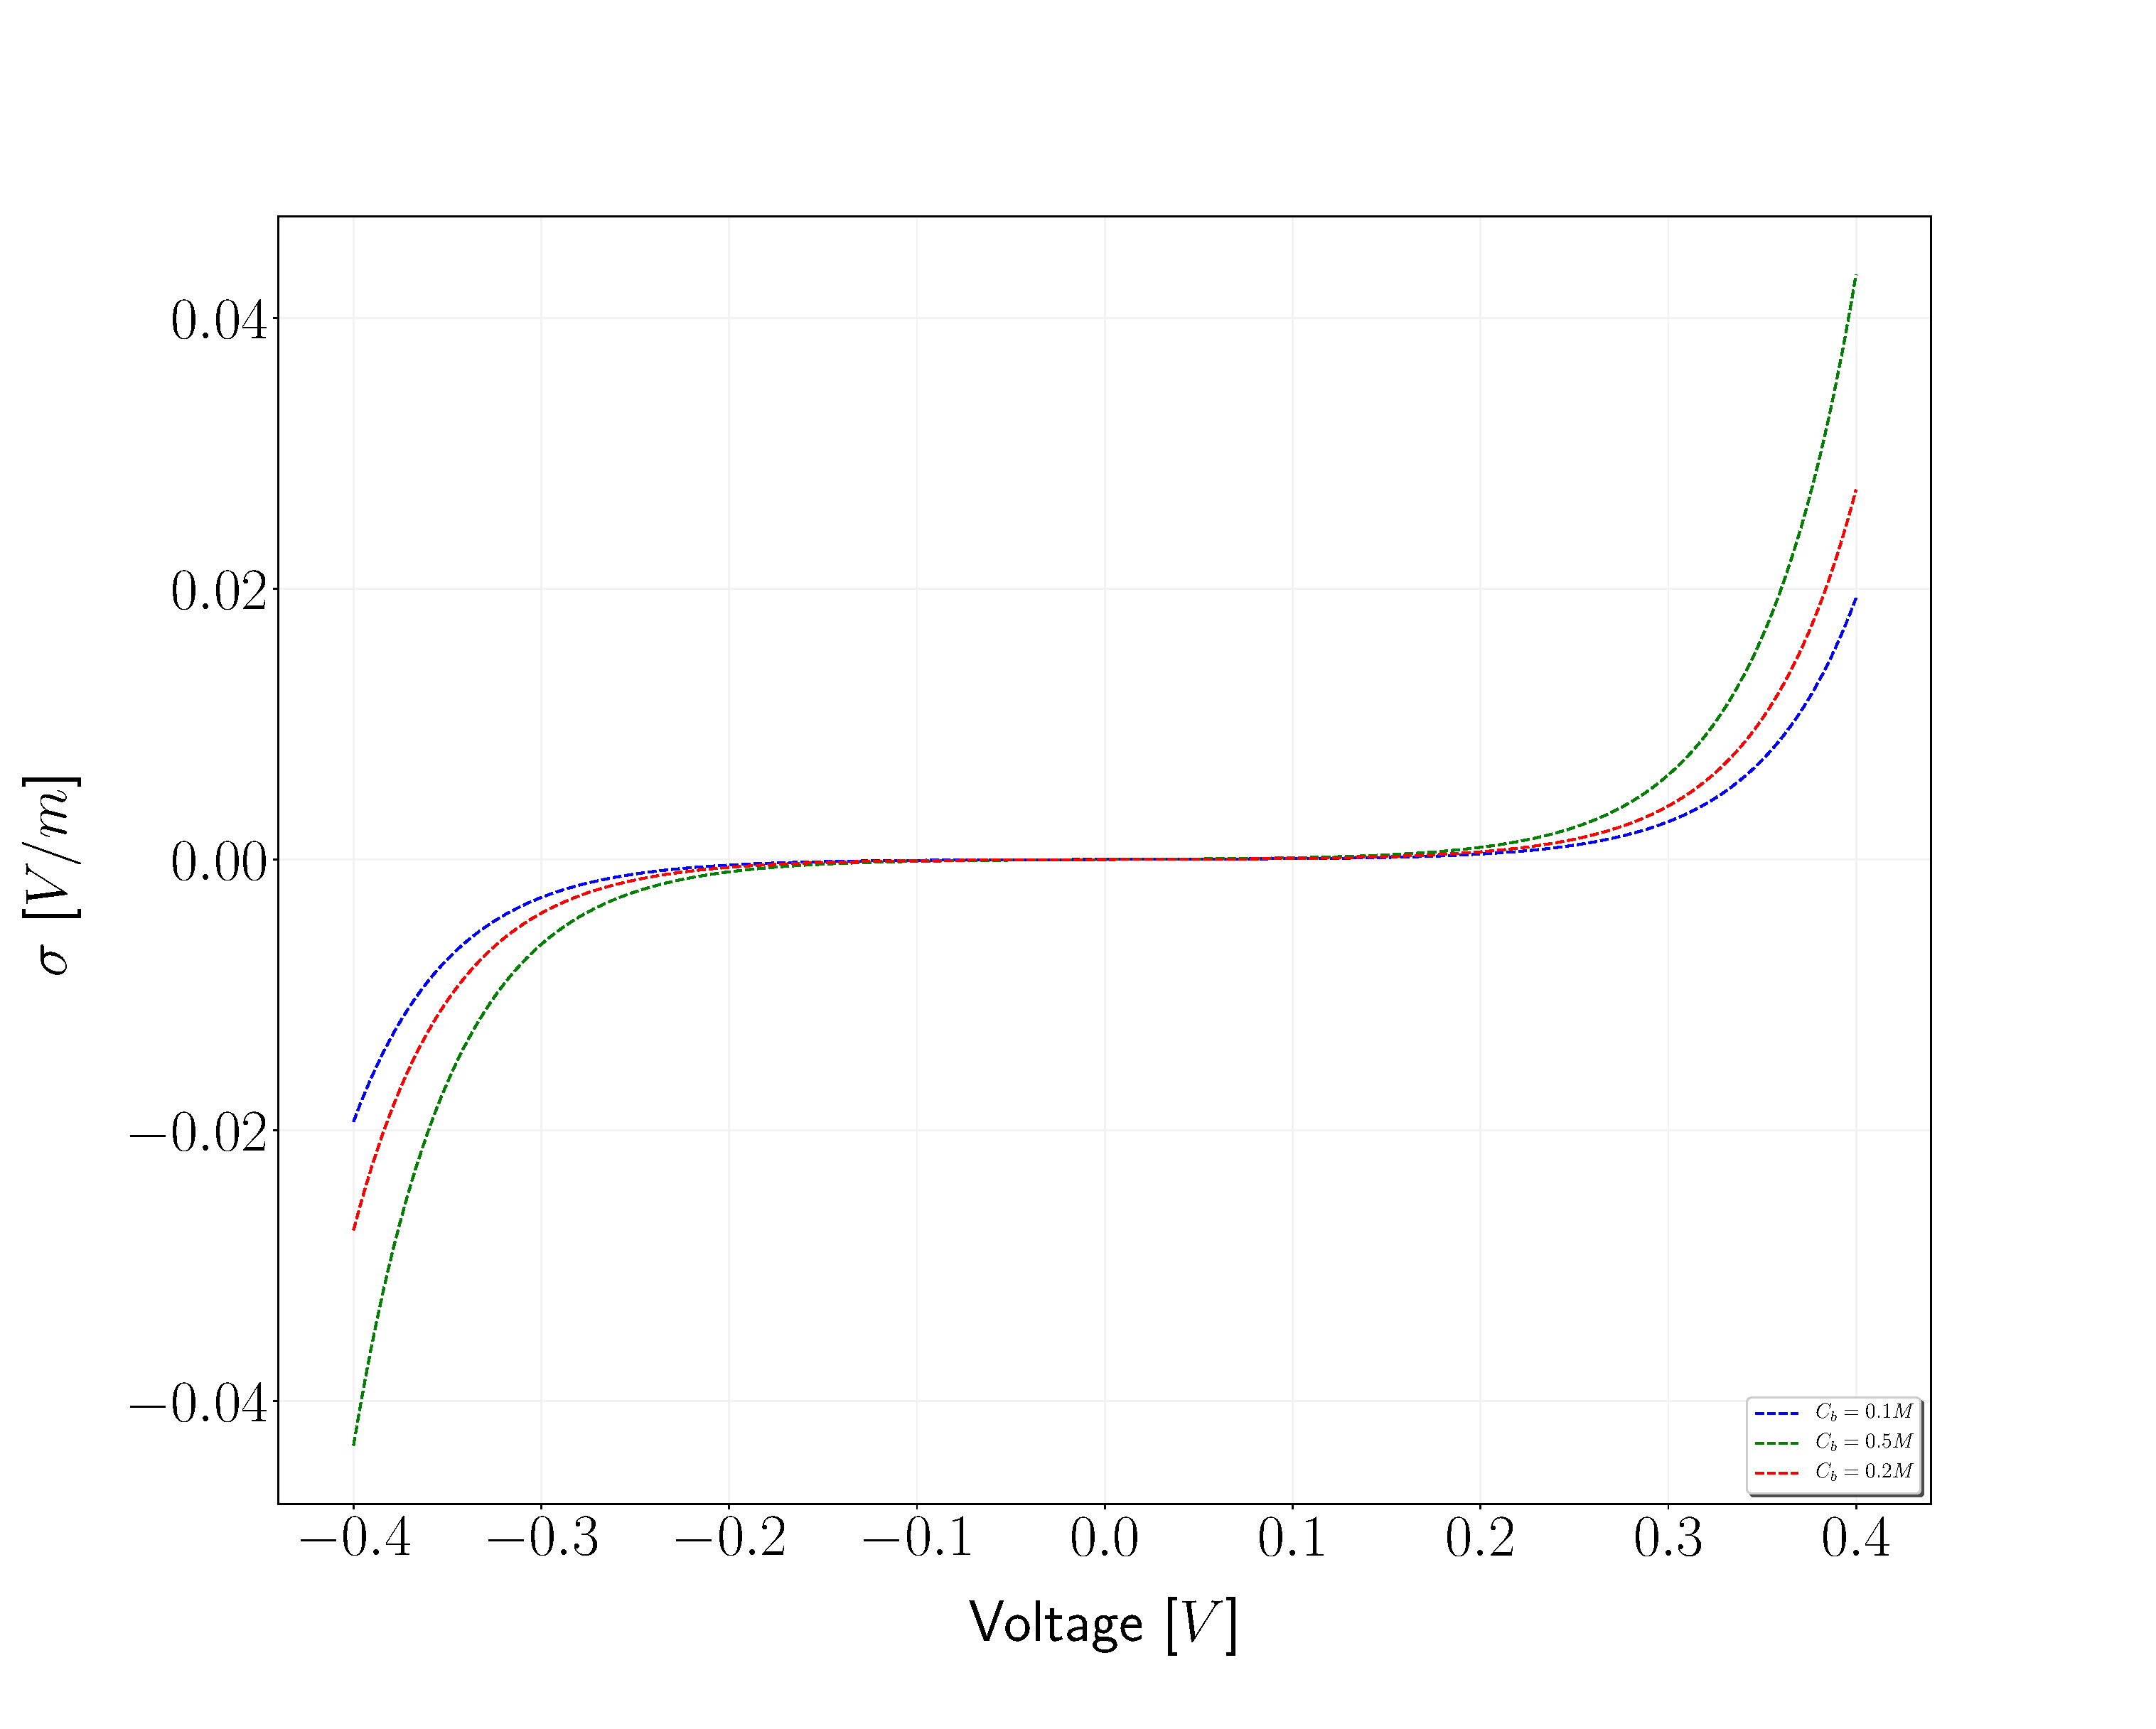
\includegraphics[width=\linewidth]{sigma-voltage.eps}
  \caption{}
  \label{fig:sub1}
\end{subfigure}%
\begin{subfigure}{.4\textwidth}
  \centering
  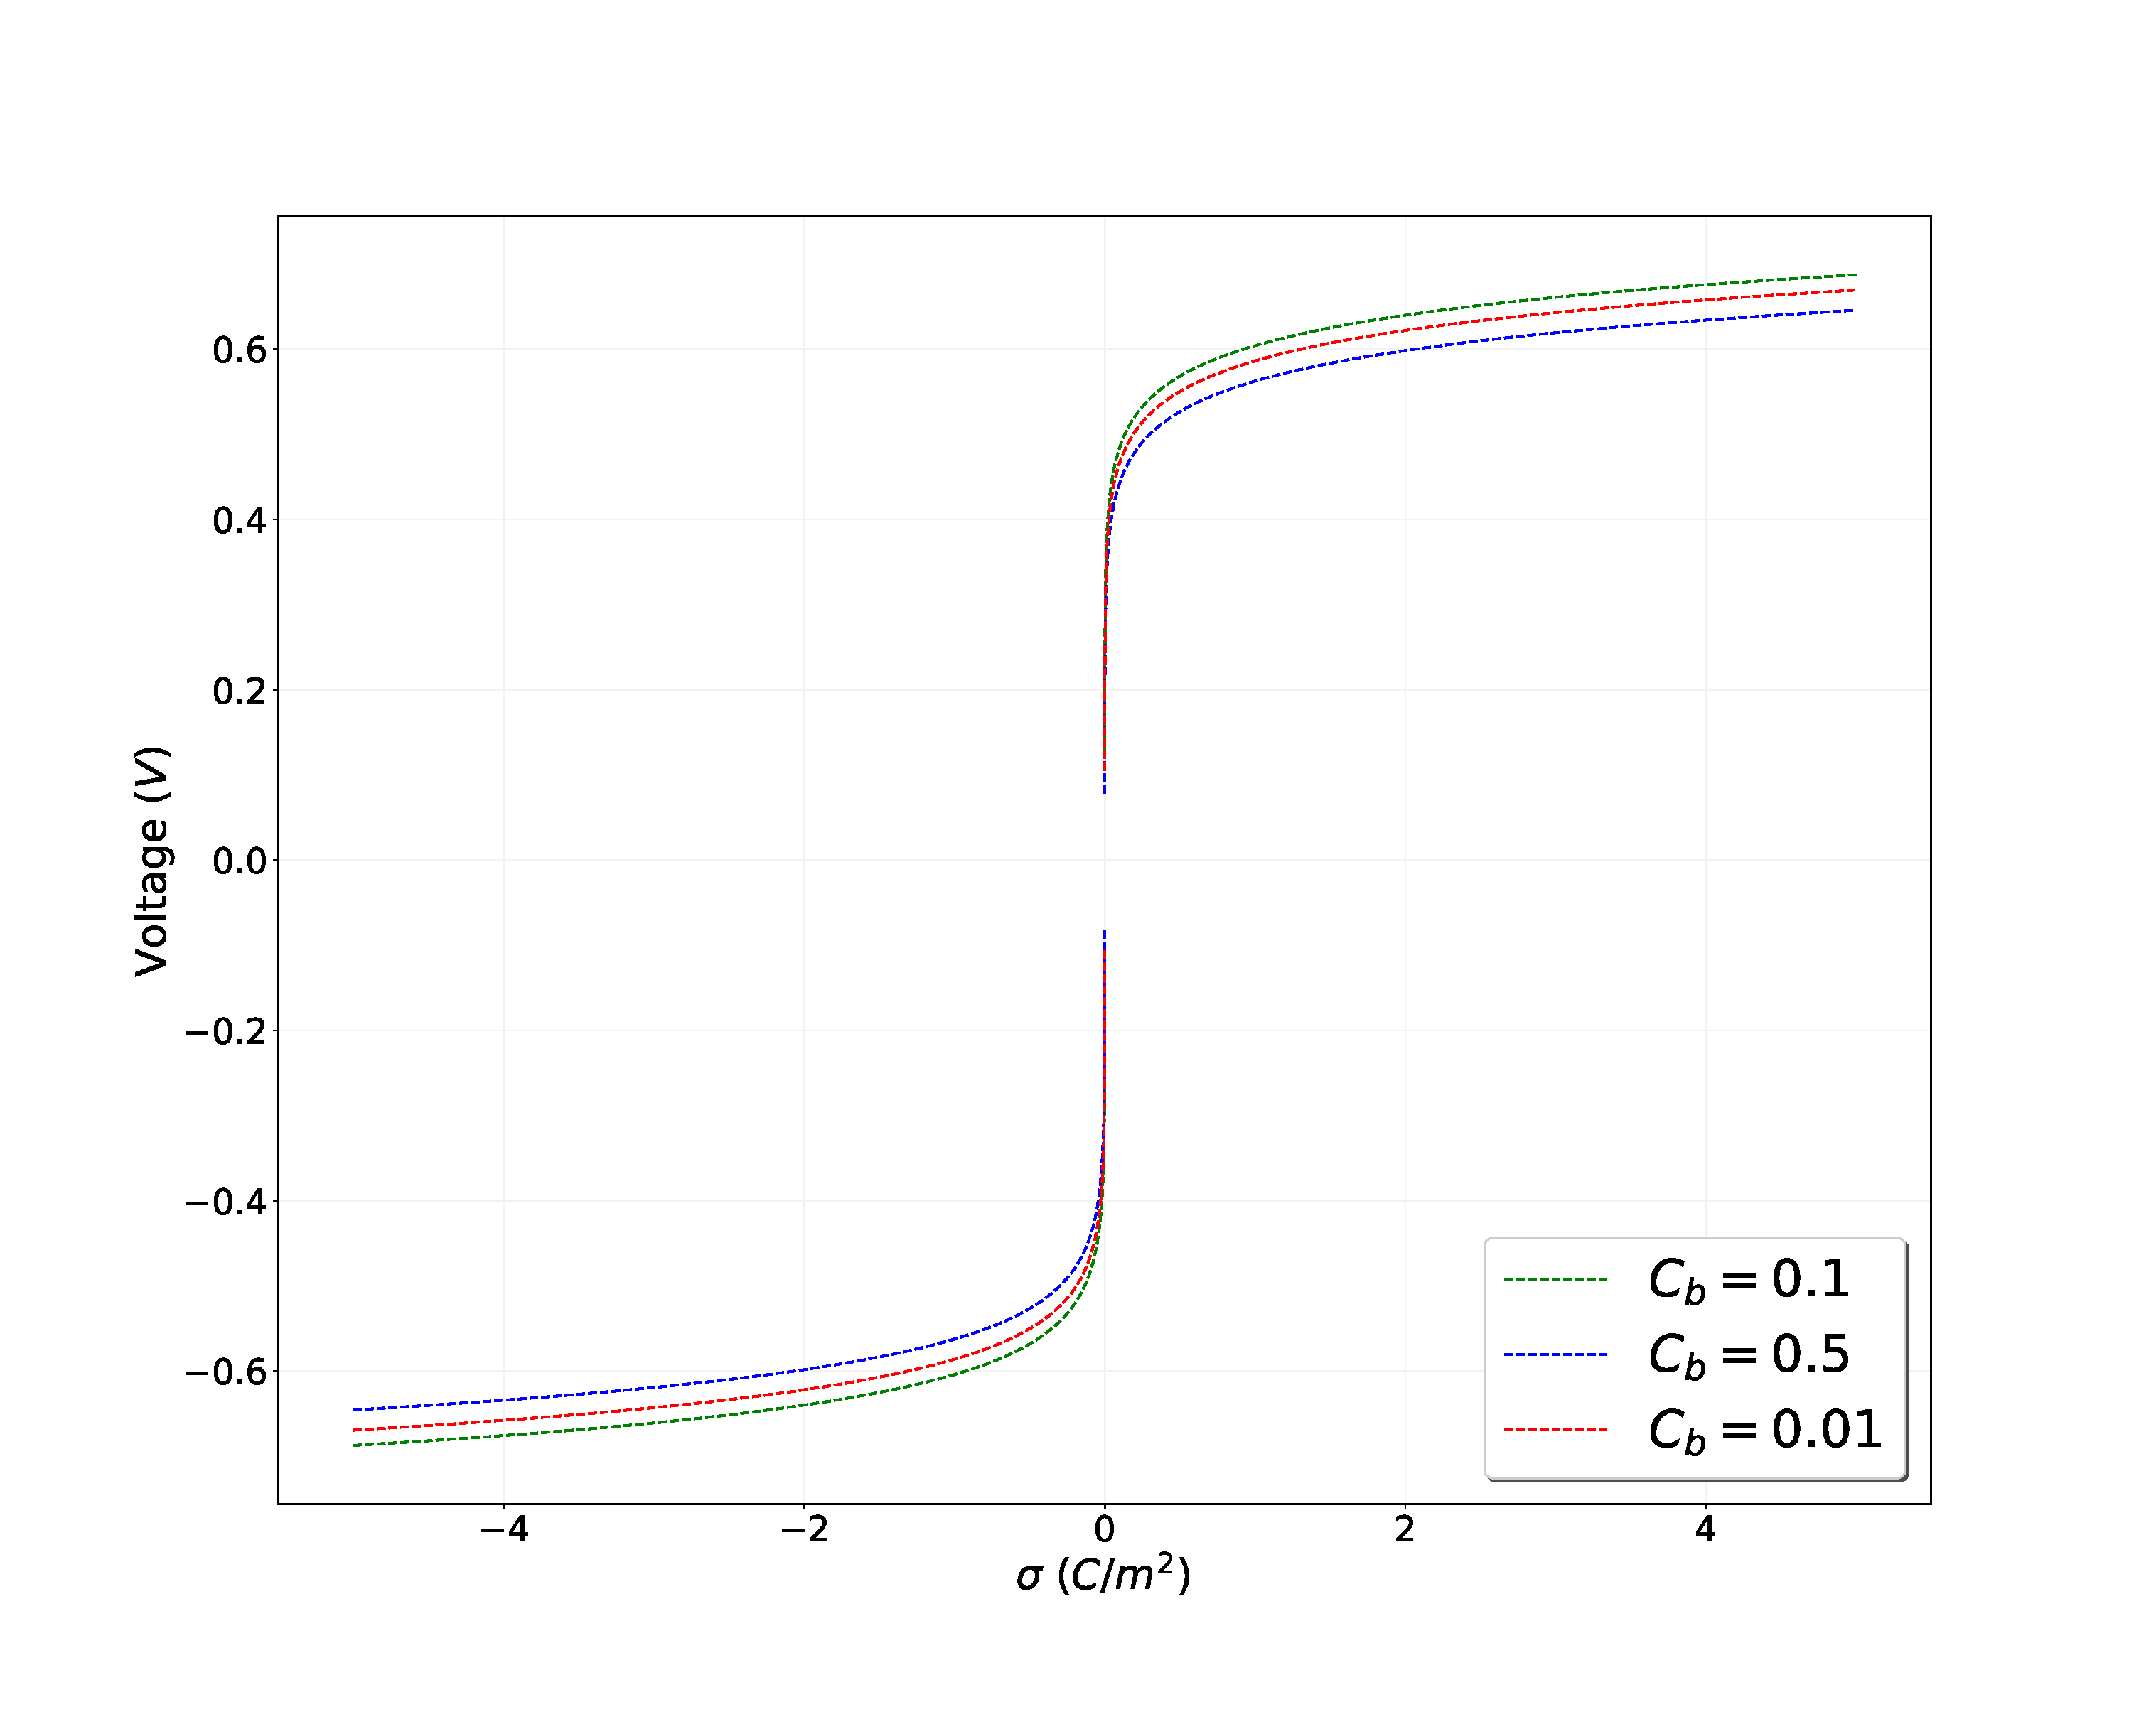
\includegraphics[width=\linewidth]{voltage-sigma.eps}
  \caption{}
  \label{fig:sub2}
\end{subfigure}
\caption{\textbf{(a)} Surface charge density in terms of the potential border condition. \textbf{(b)} Inverse of (a)}
\label{fig:test}
\end{figure}

\begin{figure}[htbp!]
\centering
\begin{subfigure}{.4\textwidth}
  \centering
  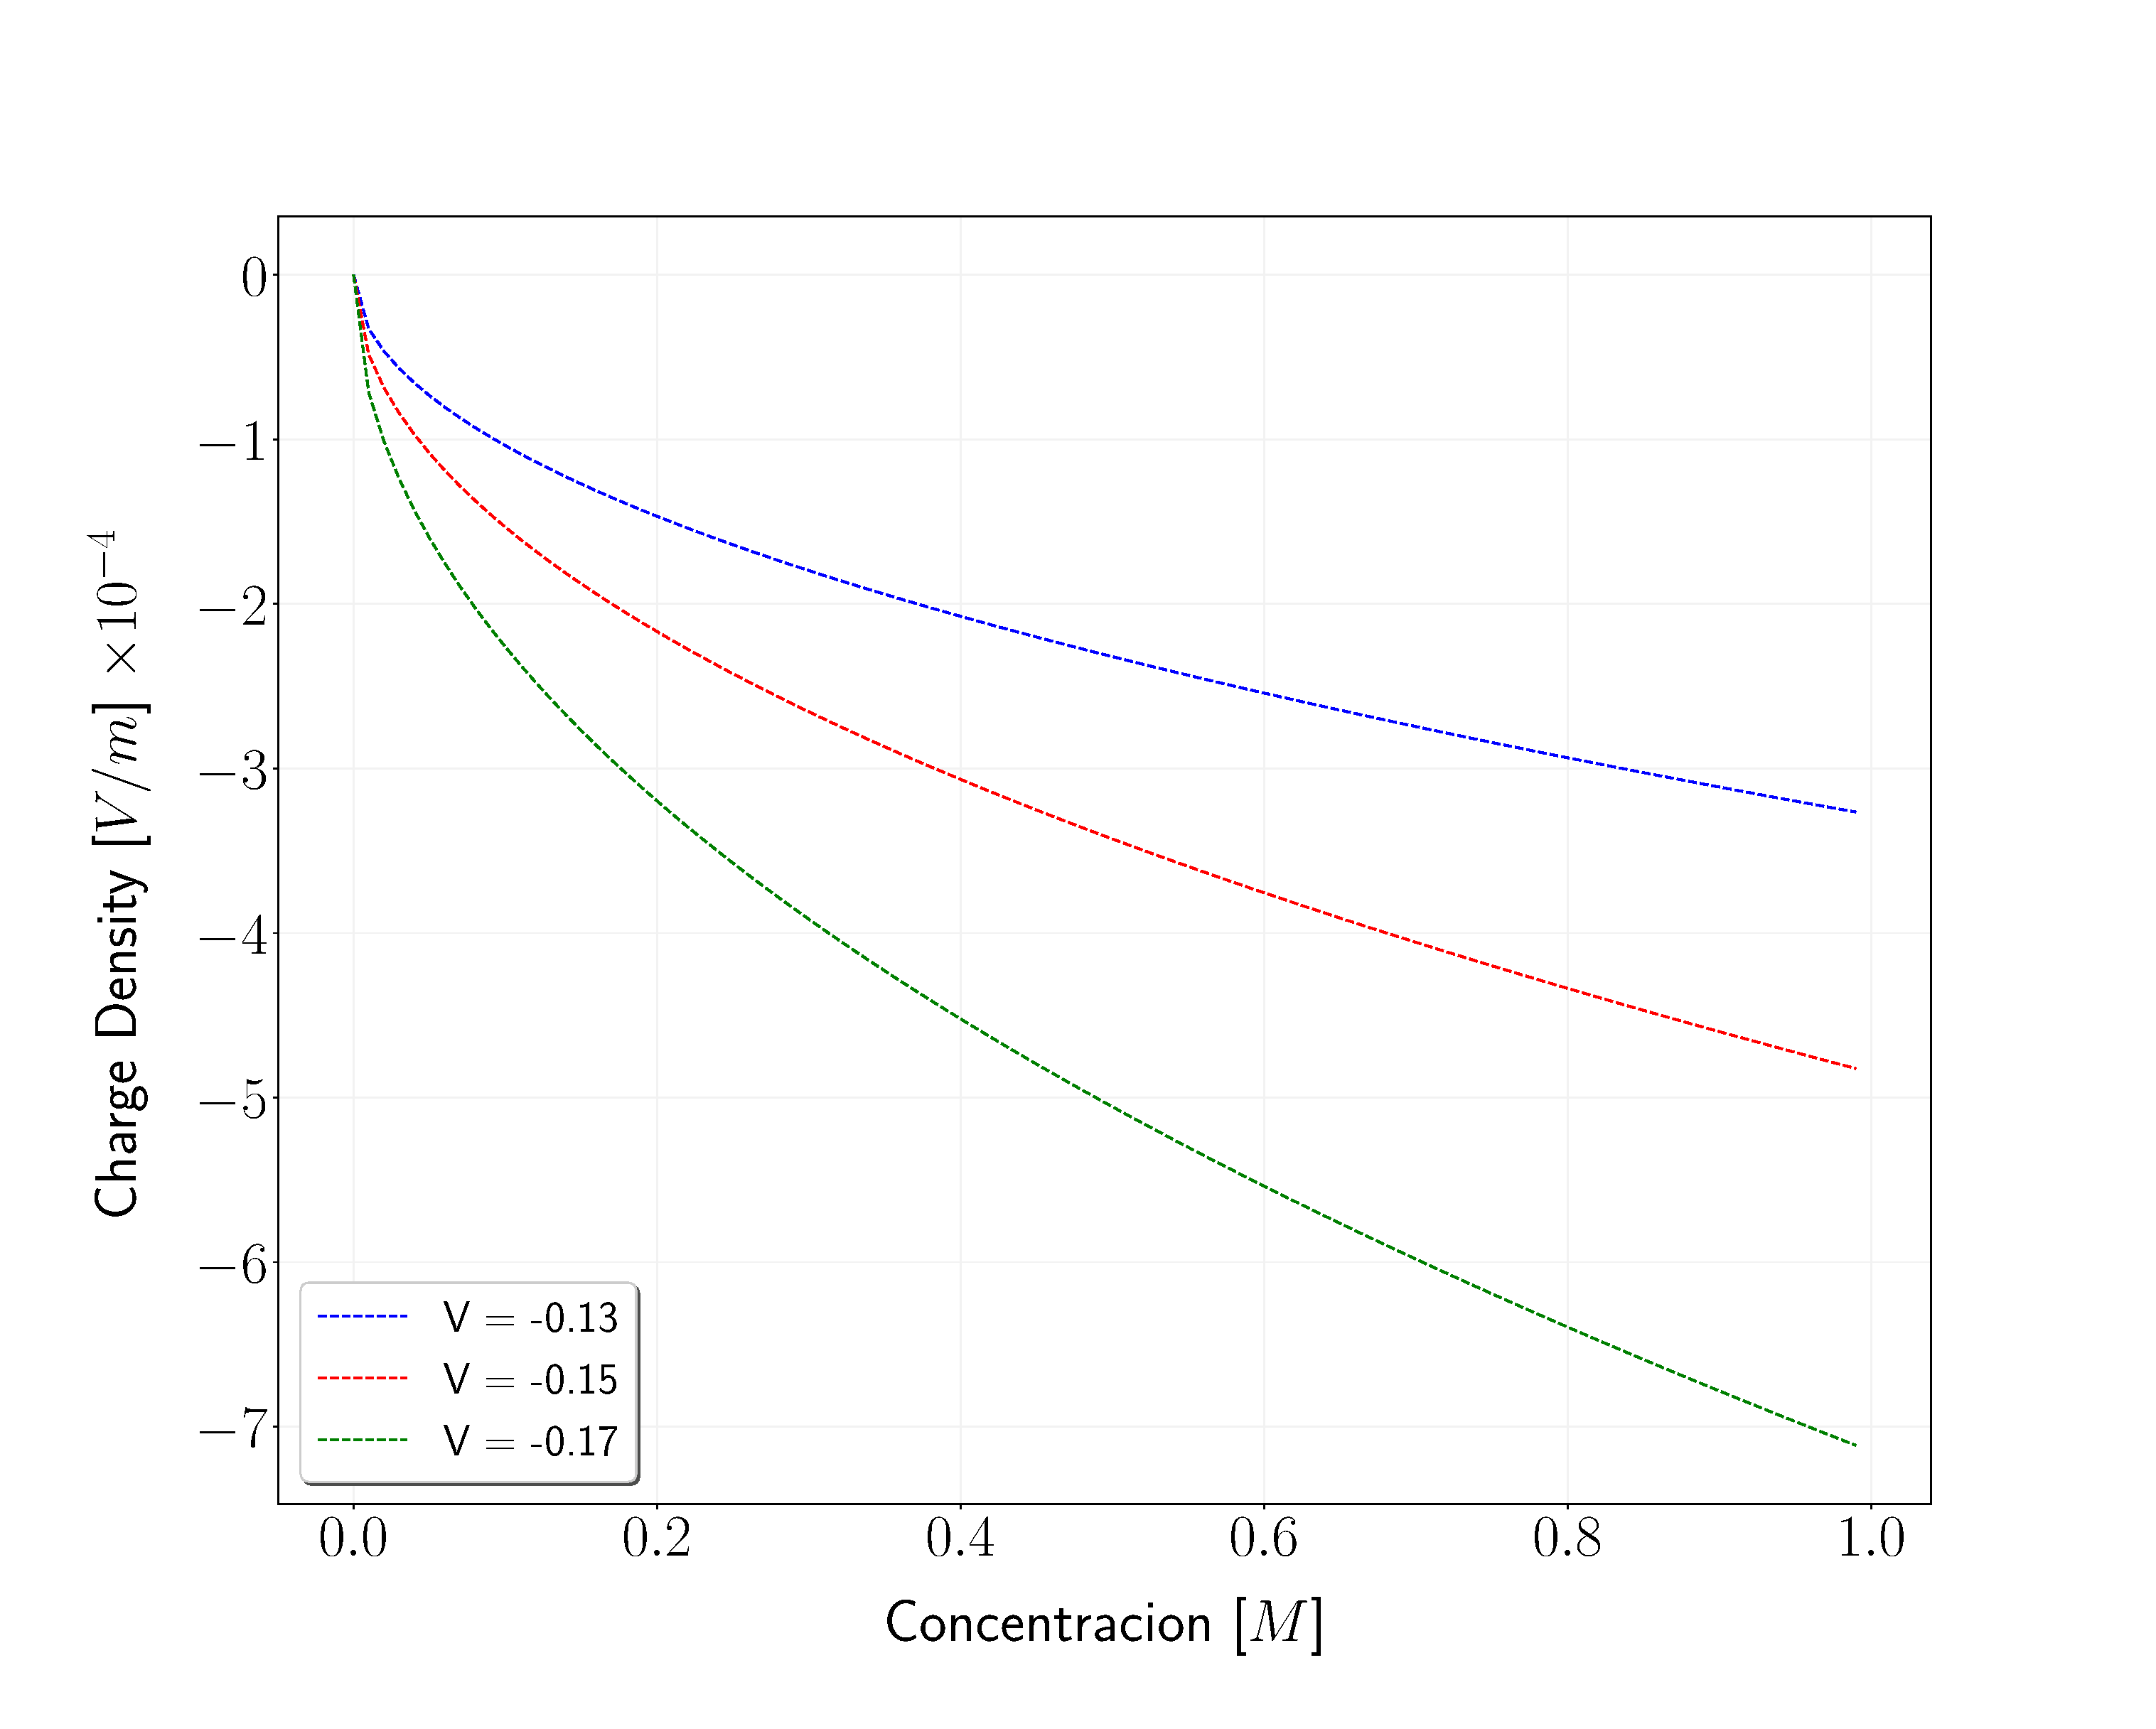
\includegraphics[width=\linewidth]{sigma-concentration.eps}
  \caption{}
  \label{fig:sub1}
\end{subfigure}%
\begin{subfigure}{.4\textwidth}
  \centering
  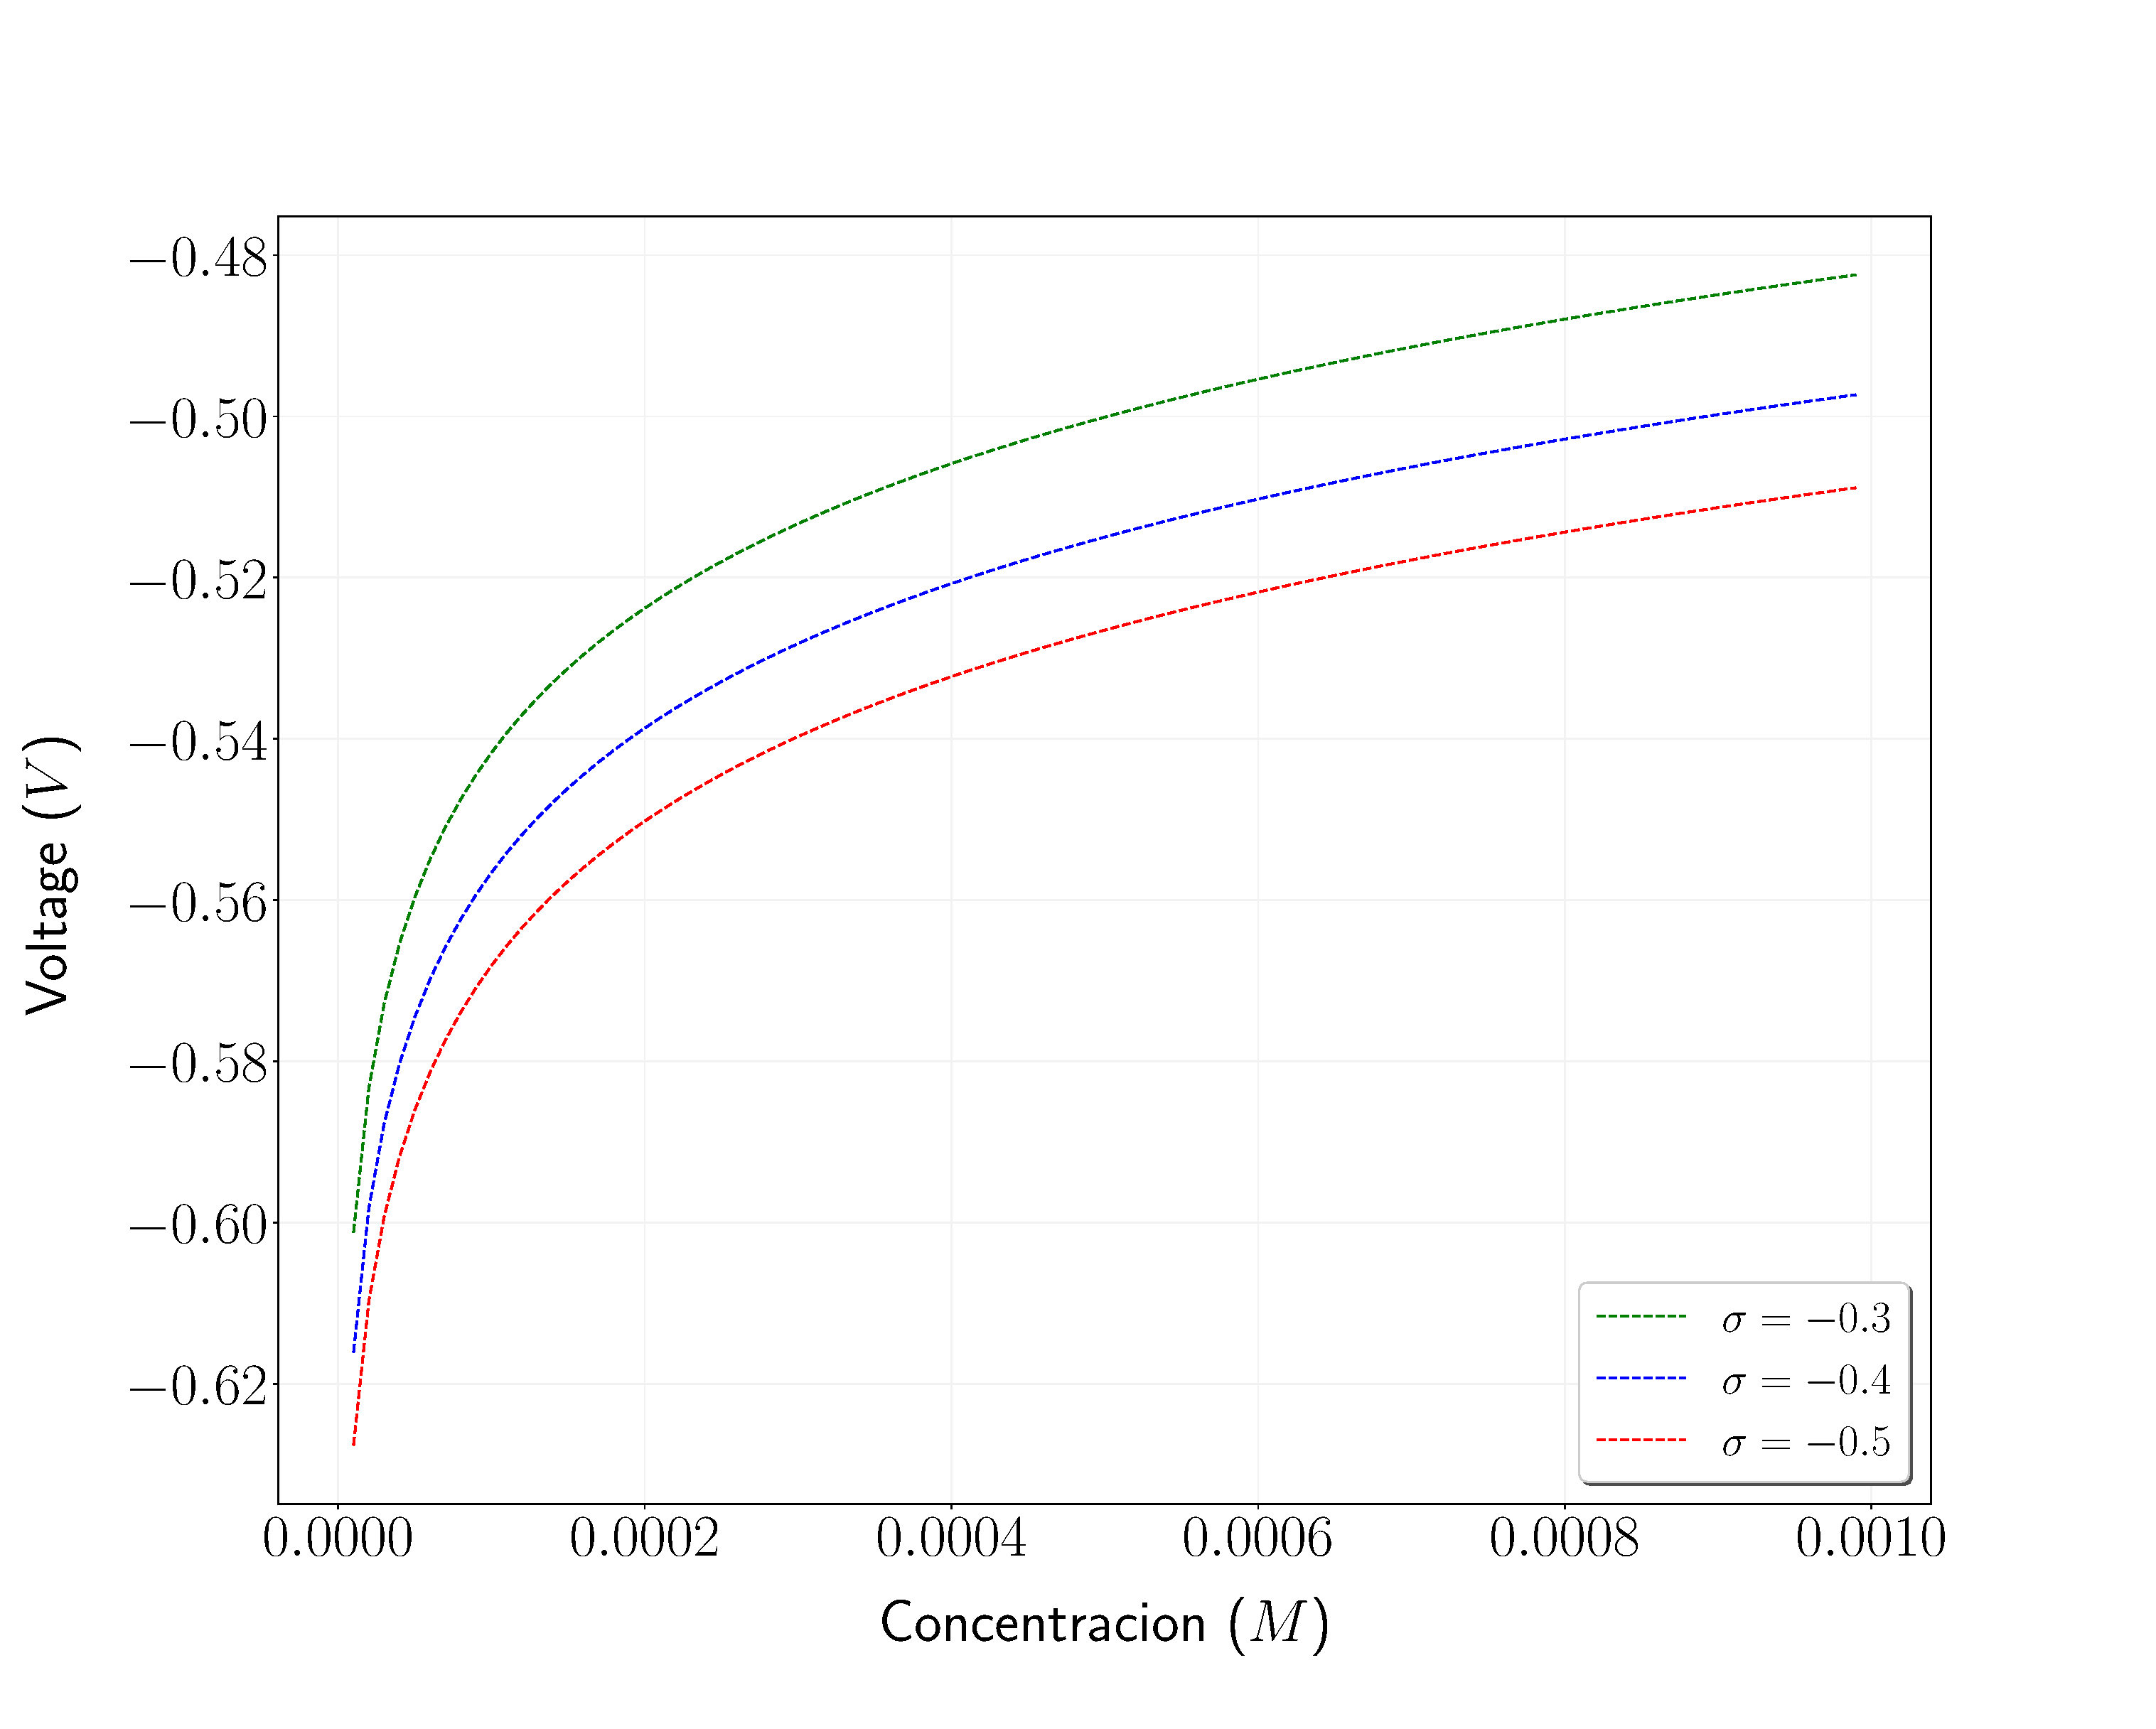
\includegraphics[width=\linewidth]{voltage-concentration.eps}
  \caption{}
  \label{fig:sub2}
\end{subfigure}
\caption{\textbf{(a)} Surface charge density in terms of the bulk concentration. \textbf{(b)} Voltage at the interface in terms of the bulk concentration (a)}
\label{fig:test}
\end{figure}




\section{Solution to the concentration at first order in the current $I_0$}


Now we solve Equation \ref{eq:system} at first order in the current $I_0$. From Eq. \ref{eq:concentration-diff-first2}, we consider the term proportional to $\frac{\partial \phi^{(1)}}{\partial x}$ such that

\begin{equation}
\bigg|\frac{\partial \phi^{(1)}}{\partial x}\bigg| << \frac{\kappa V_0}{r},
\label{eq:approx}
\end{equation}

since the gradient of the correction to the potential should be negligible compared to the gradient of the zero order contribution. This will be shown later in a numerical analysis. With this approximation, the system to first order in $r$ becomes

\begin{eqnarray}
\frac{\partial C^{(1)}_+}{\partial \xi}-C^{(1)}_+(\xi)\frac{\partial \Phi^{(0)}}{\partial \xi} &=& -\frac{1}{\kappa} \\
\label{eq:concentration-diff-first4}
\frac{\partial C^{(1)}_-}{\partial \xi}+C^{(1)}_-(\xi)\frac{\partial \Phi^{(0)}}{\partial \xi} &=& 0 \\
\label{eq:concentration-diff-first5}
\frac{\partial^2  \phi^{(1)}}{\partial \xi^2} &=& -(C^{(1)}_{+}(\xi)-C^{(1)}_{-}(\xi))
\label{eq:concentration-diff-first6}
\end{eqnarray}


In Eq. \ref{eq:concentration-diff-first4}, we obtain

$$\frac{\partial C^{(1)}_+}{\partial \xi}-C^{(1)}_+\frac{\partial \Phi^{(0)}}{\partial \xi} = -\frac{1}{\kappa}$$

Using an integrating factor of the form
$$\mu(\xi)=e^{-\int_{\kappa\delta}^\xi \frac{zF}{RT}\frac{d\phi^{(0)}}{d\xi'}d\xi'}=e^{- (\Phi^{(0)}(\xi)-\phi_b)} = e^{-\Phi^{(0)}(\xi)}$$

We can write \ref{eq:concentration-diff-first4}  as

$$\frac{d}{d\xi}\left(C^{(1)}_+(\xi)\mu(\xi) \right)=-\frac{\mu(\xi)}{\kappa},$$

where $z=|z_\pm|$. Integrating over $x$ and considering that $C^{(1)}_+(\xi)\mu(\xi)\big|_{\xi \rightarrow \infty} = C^{(1)}_{+,b} = 0$ due to border conditions, we get

$$C^{(1)}_+(\xi) =\frac{1}{\kappa\mu(\xi)}\int_{0}^{\xi}\mu(\xi')d\xi'$$

Eq. \ref{eq:concentration-diff-first5} can be integrated by separation of variables, and the solution is 

$$C^{(1)}_-(\xi) = C^{(1)}_{b,-}e^{\phi^{(0)}(\xi)}.$$

Since our border condition yields $ C^{(1)}_{b,-} = 0$, the contribution to first order of the negative ion concentration is zero. 

Computing the integral, we find to first order in the current the following solutions for the concentrations.

\begin{eqnarray}
C^{(1)}_+(\xi) &=& -\frac{1}{\kappa} \qty{\xi_\delta-\xi-\frac{2}{\gamma}}\tanh^2\qty{\frac{\xi-\xi_0}{2}}+2\tanh\qty{\frac{\xi-\xi_0}{2}}\\
C^{(1)}_-(\xi) &=& 0
\label{eq:firstordersol}
\end{eqnarray}



\section{Potential to first order in the current}

Now we need to solve Eq. \ref{eq:concentration-diff-first6}
\begin{eqnarray}
\frac{\partial^2  \Phi^{(1)}}{\partial \xi^2} &=& -(C^{(1)}_{+}(\xi)-C^{(1)}_{-}(\xi)).
\end{eqnarray}

Expanding, we have 

\begin{eqnarray}\nonumber
\frac{\partial^2  \Phi^{(1)}}{\partial \xi^2} &=& -C^{(1)}_{+}(\xi)\\
&=& -\frac{1}{\kappa} \qty{\xi_\delta-\xi-\frac{2}{\gamma}}\tanh^2\qty{\frac{\xi-\xi_0}{2}}+2\tanh\qty{\frac{\xi-\xi_0}{2}}
\end{eqnarray}


Integrating twice and using the fact that $\Psi'^{(1)} = 0$, $\Psi^{(1)} = 0$ we obtain

\begin{eqnarray}
\Phi'^{(1)}(\xi) = \frac{1}{\kappa} \qty{A + B\xi + C\xi^2 + D \tanh{\frac{\xi-\xi_0}{2}}+E\xi\tanh{\frac{\xi-\xi_0}{2}}} 
\end{eqnarray}


And 

\begin{eqnarray}
\Phi^{(1)}(\xi) = -\frac{1}{\kappa} (A(\xi_\delta - \xi) + \frac{B}{2}(\xi_\delta^2-\xi^2) + \frac{C}{3}(\xi_\delta^3 - \xi^3) + \\
D\log\bigg|\frac{\cosh{\frac{\xi_\delta-\xi}{2}}}{\cosh{\frac{\xi-\xi}{2}}}\bigg| + E \qty{\xi_\delta\log|\cosh\qty{\frac{\xi_\delta-\xi_0}{2}}-\xi\log|\cosh\qty{\frac{\xi-\xi_0}{2}}}-EI_\delta(\xi)
\end{eqnarray}


where

\begin{eqnarray*}
	A = 2\gamma\xi_\delta - \frac{2\xi_\delta}{\gamma} - 2 \gamma - \frac{\xi_\delta^2}{2},\\
	B = -\qty{\xi_\delta -\frac{2}{\gamma}},\\
	C = \frac{3}{2}\\
	D = -2 \qty{\xi_\delta - \frac{2}{\gamma}},\\
	E = 2,\\
	\gamma = \tanh\qty{\frac{\xi_0}{2}},
\end{eqnarray*}

and

\begin{align}
	I_\delta(\xi) = \int_\xi^{\xi_\delta} \log\bigg|\cosh\qty{\frac{\xi-\xi_0}{2}}\bigg| d\xi.
\end{align}




This integral must be evaluated numerically for each value of $\xi$. In order to do this, we use the Simpson Rule. Fig. \ref{fig:analytic-results} shows the potential to first order in the current alongside with the zero order potential. 


\begin{figure}[h!]
 \centering
 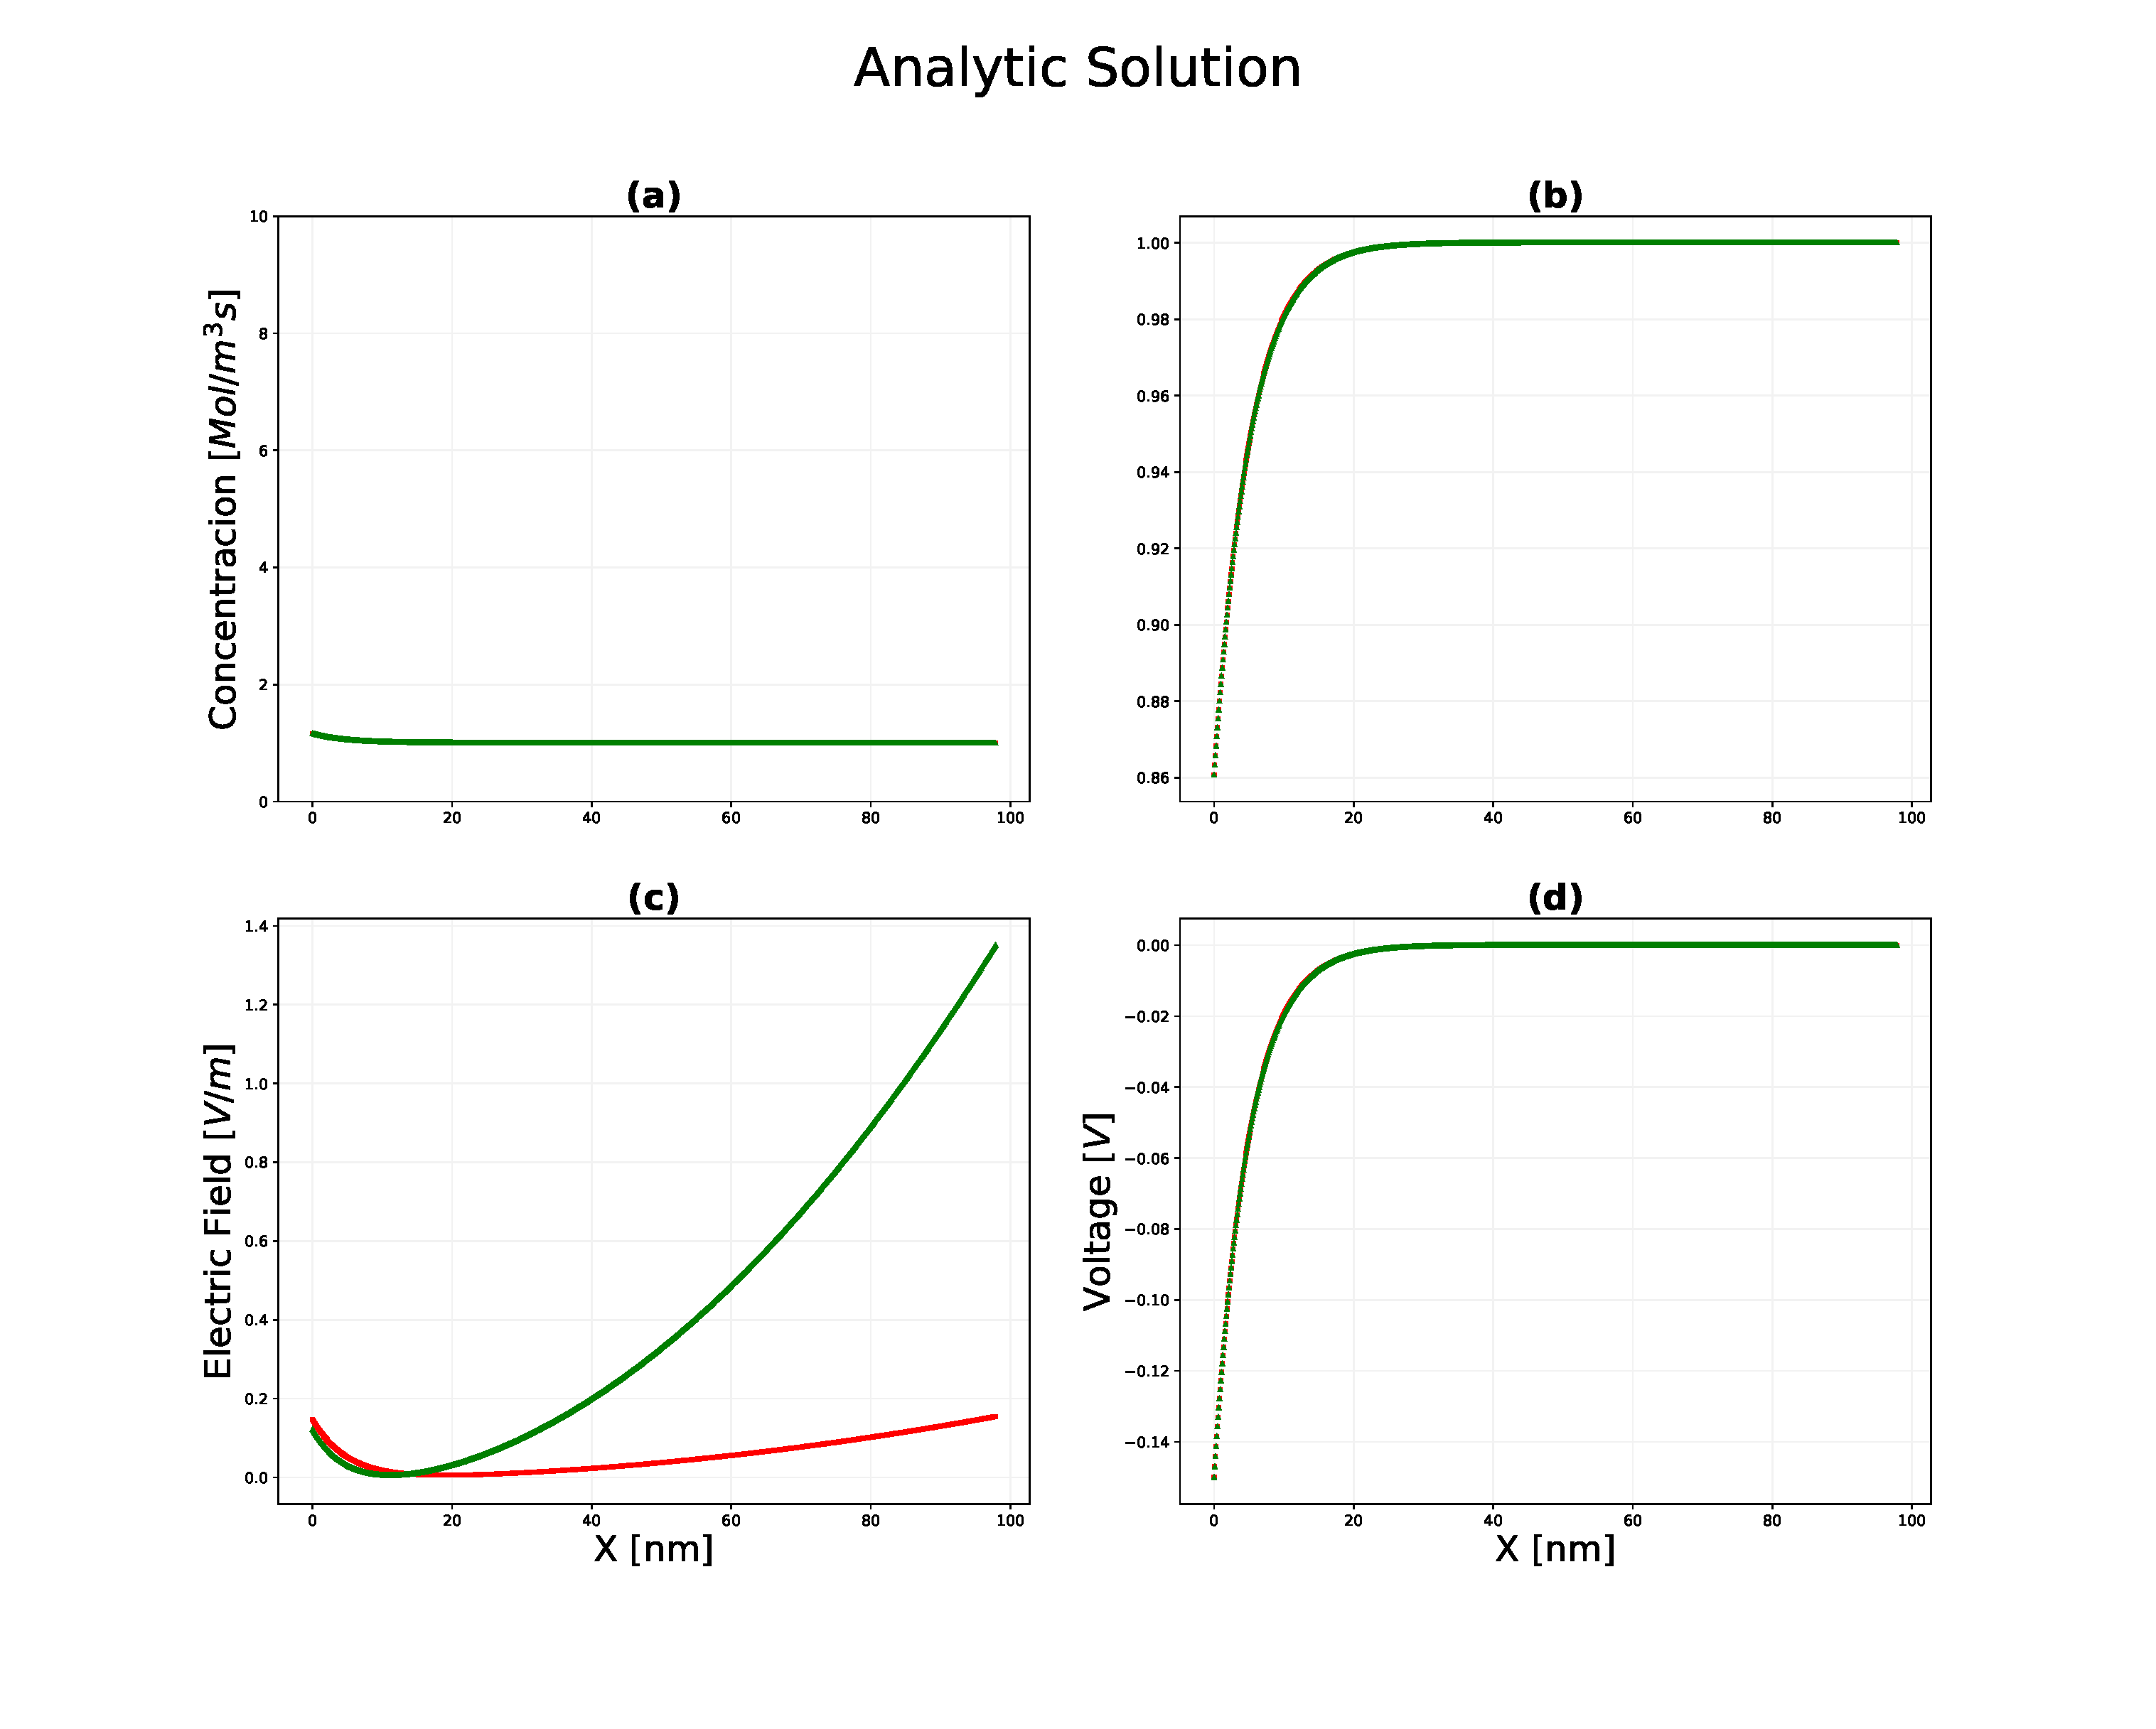
\includegraphics[width = \linewidth]{analytic-results}
 \caption{Analytic results. (a), (b) are the concentrations of each species of electrolytes. (c) is the electric potential and (d) the electric potential. Each plot is compared for 3 different values of the reactio rate.}
 \label{fig:analytic-results}
\end{figure}







\section{Numerical Analysis}

In order to validate the approximations made in previous sections, we solve system \ref{eq:system} numerically. In order to do so, we use the Runge-Kutta Method of order 4 along with the  Shooting Method to solve the two point boundary value (reference to Numerical Methods in python).  



The complexity of the problem lies exactly in the two point boundary feature of the problem, where the concentrations are known in the bulk, but the potential is known at the interface(see Fig. \ref{fig:geometry}). 

The approach used in these type of problems is transforming the second order system \ref{eq:system} into a first order one,

\begin{eqnarray}
C'_+(x)-\frac{zF}{RT}E(x)C_+(x) &=& -r, \\
C'_-(x)+\frac{zF}{RT}E(x)C_-(x) &=& 0, \\
E'(x) &=& \frac{zF}{\epsilon}(C_+(x)-C_-(x)), \\
\phi'(x) &=& -E(x).
\label{eq:linear-system}
\end{eqnarray}

subject to the border conditions

\begin{eqnarray}
C_+(\delta) &= C_b,  \\
C_-(\delta) &= C_b, \\
\phi(\delta) &=& 0\\
\phi(0) &=&  V_0
\label{eq:linear-system}
\end{eqnarray}

Here the primes denote derivatives with respect to $x$. Once the system is in the form of Eqn. \ref{eq:linear-system}, we can apply the Runge-Kutta Method with the shooting method to obtain the numerical solutions. 


\section{Results}

Fig. \ref{fig:numeric-results} show the results obtained. The solution of the steady state at different values of the reaction rate do not defer much closest to the surface of the electrode ($x=0$). Also, from Fig. \ref{fig:numeric-results} (c) and (d) we can see that the aproximation of the electric field and the electric potential is fairly 

\begin{figure}[htbp]
 \centering
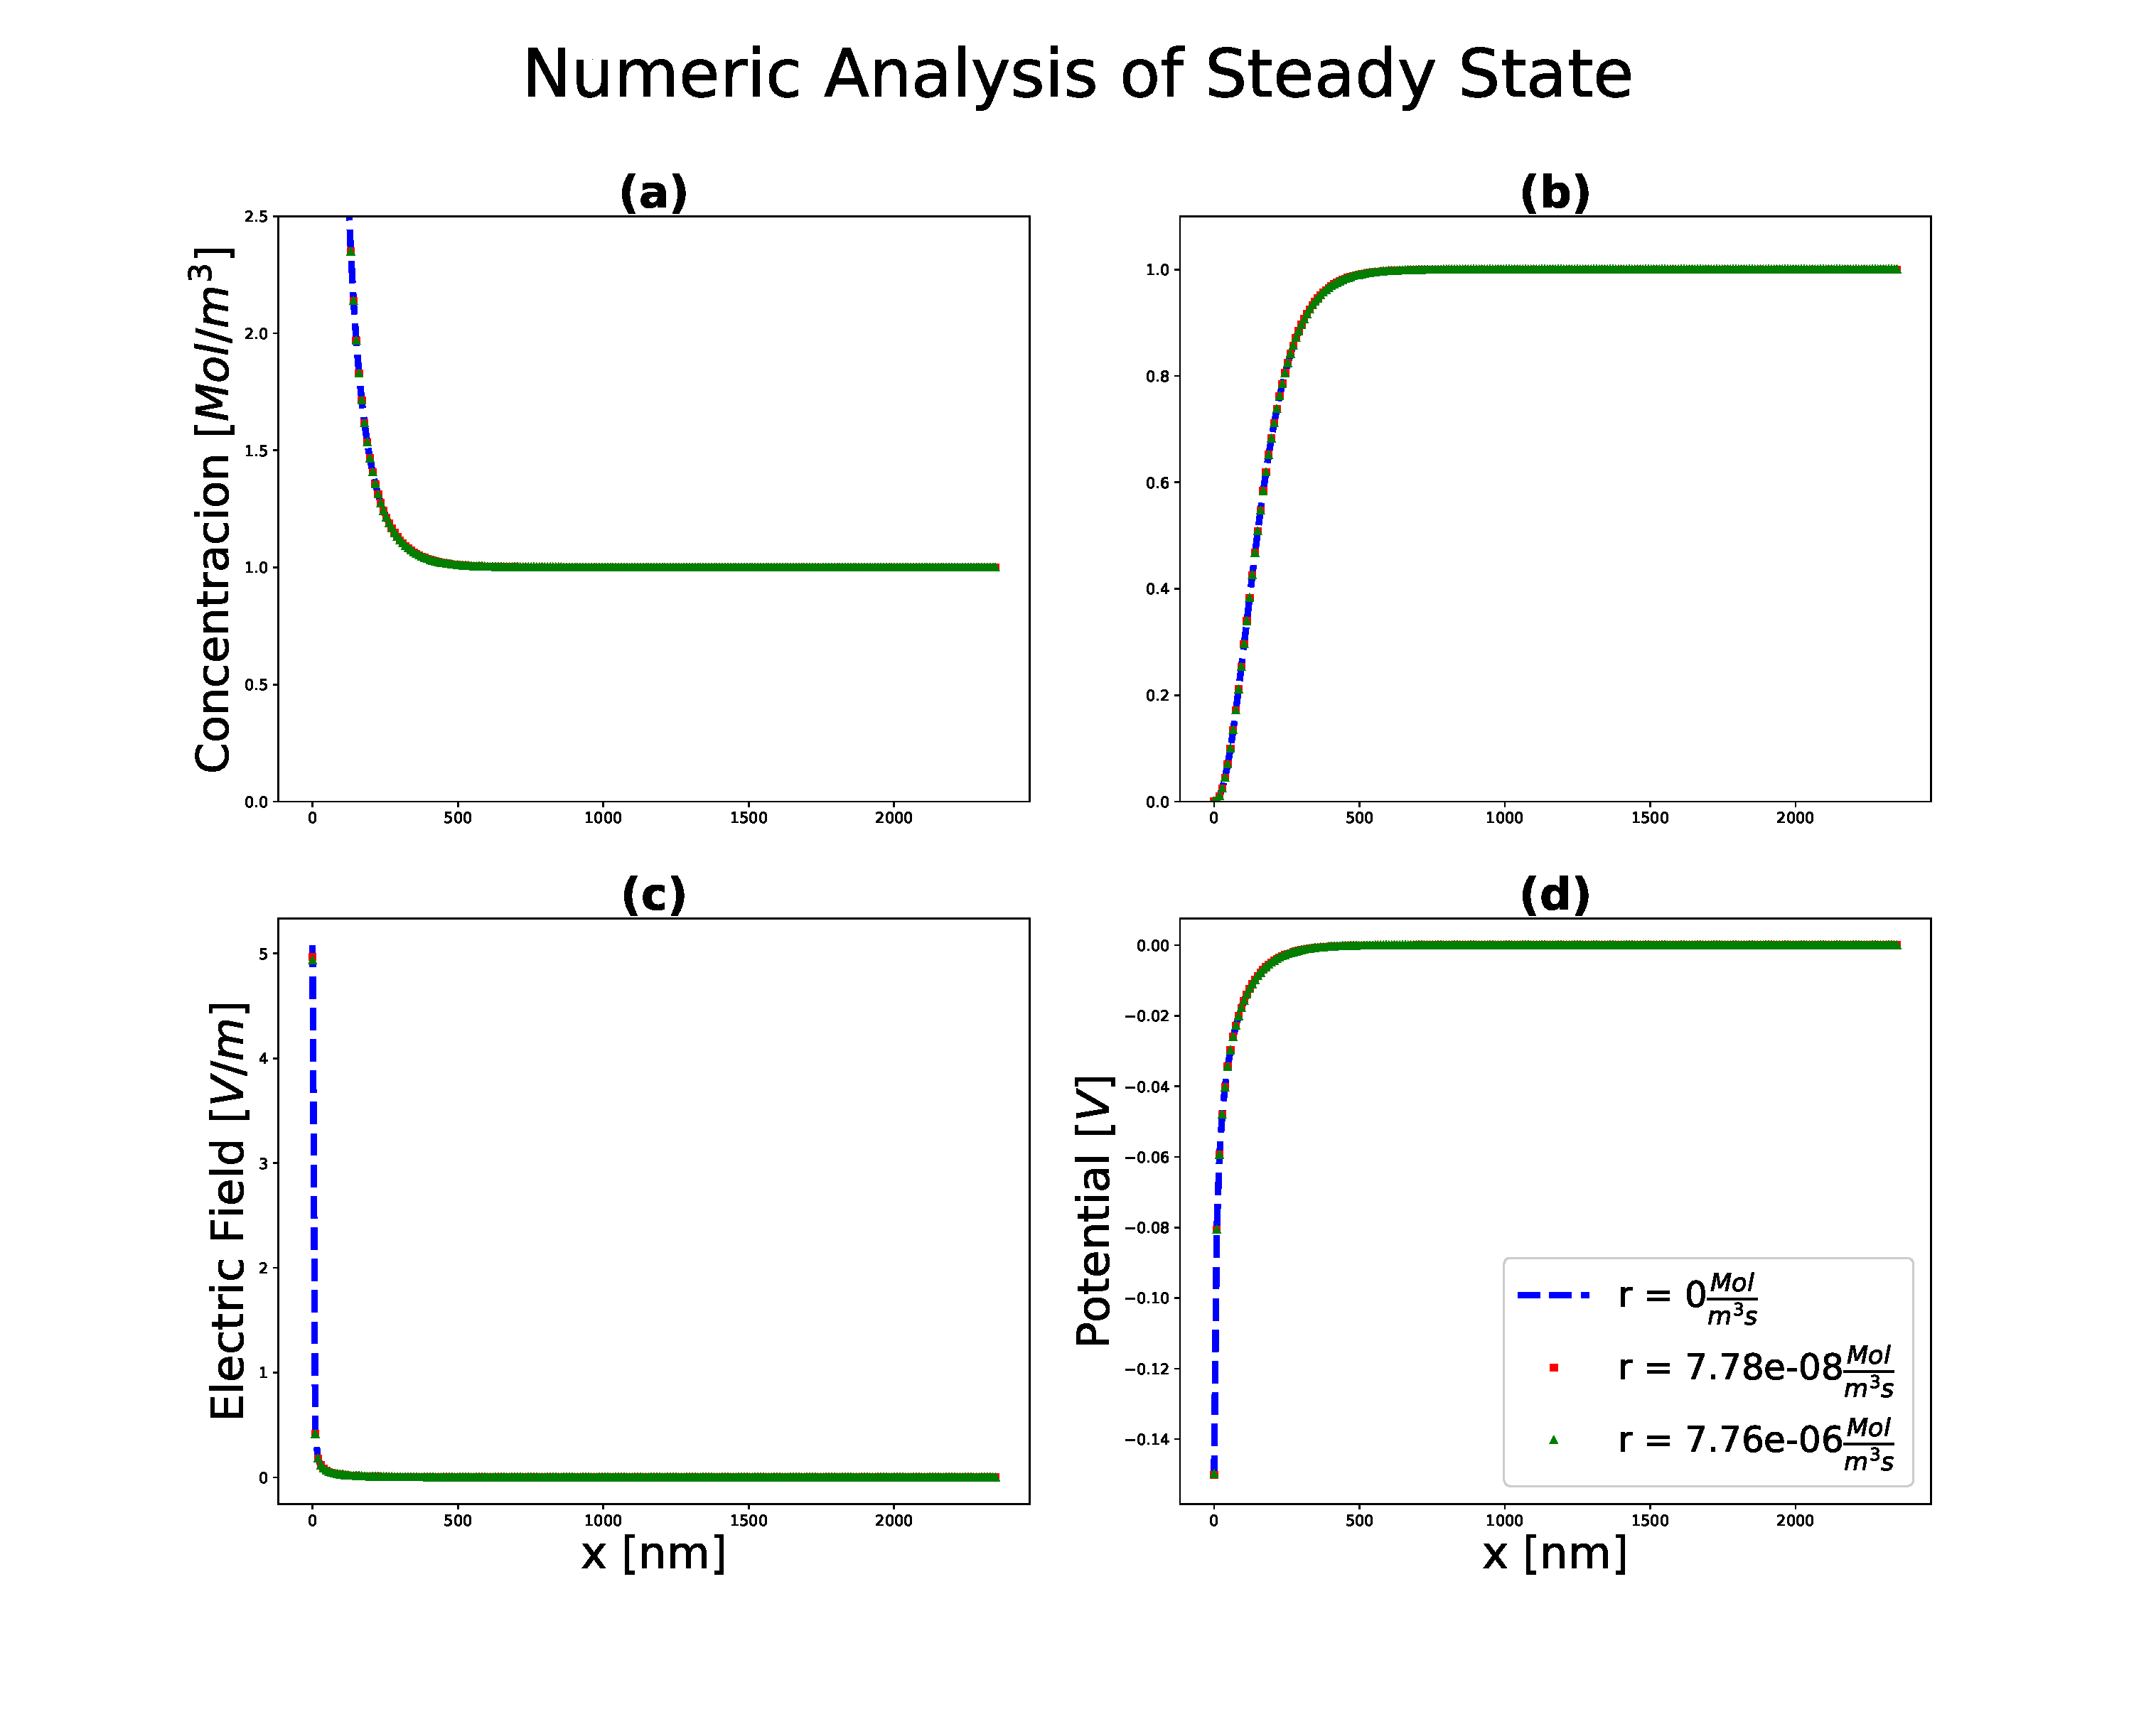
\includegraphics[width = \linewidth]{results-numeric}
 \caption{The numerical and the analytic solution to the potential to first order in the current.}
 \label{fig:numeric-results}
\end{figure}

Dealing with the equations as presented in Eq. \ref{eq:system} is extremely difficult when doing a numerical analysis. This is due to the fact that the natural units of the system (x which is measured in meters) are too small for the computer to handle. Also, non-linearity gives extreme fluctuations of the concentration of the positive ion near the surface. Since we where using the shooting method, we needed to change the values of the electric field at the bulk, such that the boundary condition for the electric potential is correct, but this induced such strong concentrations at the interface sometimes, that the computer could not handle the numbers resulting from Runge-Kutta method. We had to make a little adaptation in order to be able to find the correct boundary condition for the electric field with the shooting method. 




As it can be seen in figures  \ref{fig:numerical-phi},  \ref{fig:numerical-E}, the electric field and potential approach zero when the start moving into the bulk of the solution, as expected. The further away from the interface we go, the better the border conditions for the electric field are met. For our particular case, we cut the integration range when we reached a tolerance of $ E_{bulk} < 1\times 10^{-3}$, where $E_{bulk}$ is the border condition of the dimensionless electric field at the bulk. 



A similar analysis can be done for the concentrations (Fig.  \ref{fig:numerical_c}), but this time the value of both concentrations at the bulk is $C_b$, as defined by the border conditons for the system \ref{eq:system}.



Another difficulty is that, since we used the adaptive Runge-Kutta method, the concentrations change so abruptly that the adaptive step $h$ becomes increadibly small. The problem with this is that the number of iterations needed with a step of the order of $h\approx 10^{-29}$. In order to reach the full length of integration is too big and therefore, we obtain only a part of the integration interval and not as close to the interface as we should like. 

To avoid such difficulties, we have worked with the adimensional potential in a scale of adimensional length $\xi = \kappa x$. We have integrated on the interval $[0, 20 \kappa \delta]$.




\chapter{Dynamic Solution}
\section{Analytic Solution}

Consider know the dynamical model in which time dependence is not neglected

\begin{eqnarray}
	\frac{\partial C_+}{\partial t} = D_+\qty{\frac{\partial^2 C_p}{\partial x^2} - \frac{\partial}{\partial x}\qty{C_+\frac{\partial\Psi}{\partial x}}} \\
	\frac{\partial C_+}{\partial t} = D_+\qty{\frac{\partial^2 C_p}{\partial x^2} - \frac{\partial}{\partial x}\qty{C_+\frac{\partial\Psi}{\partial x}}} \\
	\nabla^2 \Psi = -(C_+-C_-)
\end{eqnarray}

By making the following change of variables 

\begin{eqnarray}
	\xi = \frac{\kappa x}{\sqrt{4Dt}}\\
	\frac{\partial \xi}{\partial x} = \frac{\kappa}{\sqrt{4Dt}}\\
	\frac{\partial \xi}{\partial x} = -\frac{\kappa x}{2\sqrt{4Dt^3}}
\end{eqnarray}

we can re-write the system of equations as

\begin{eqnarray}
	\label{eq:sys_dyn1}
	\frac{\partial^2 C_+}{\partial \xi^2} + \frac{2\xi}{\kappa}\frac{\partial C_p}{\partial \xi}  -\frac{\partial C_+}{\partial \xi}\frac{\partial \Psi}{\partial x}-C_+\frac{\partial^2\Psi}{\partial \xi^2} \\
	\label{eq:sys_dyn2}
	\frac{\partial^2 C_+}{\partial \xi^2} + \frac{2\xi}{\kappa}\frac{\partial C_p}{\partial \xi}  +\frac{\partial C_+}{\partial \xi}\frac{\partial \Psi}{\partial \xi}+C_+\frac{\partial^2\Psi}{\partial \xi^2} \\
	\label{eq:sys_dyn3}
	\nabla^2 \Psi + 4Dt(C_+-C_-) = 0
\end{eqnarray}

In order to solve the previous system, we will integrate equations \ref{eq:sys_dyn1} and \ref{eq:sys_dyn1}. Lets write the two equations as one in terms of the charge of the electrolyte $s=\pm$.

\begin{equation}
	\frac{\partial^2 C_s}{\partial \xi^2} + \frac{2\xi}{\kappa}\frac{\partial C_s}{\partial \xi}  -s\frac{\partial C_s}{\partial \xi}\frac{\partial \Psi}{\partial \xi}-sC_s\frac{\partial^2\Psi}{\partial \xi^2}
\end{equation}

Since,

\begin{equation}
	\int_0^\xi \frac{\partial C_s}{\partial \xi} = \xi C_s(\xi) - \int_0^\xi C_s(\xi) d\xi
\end{equation}
\begin{equation}
	\int_0^\xi \frac{\partial C_s}{\partial \xi}\frac{\partial \Psi}{\partial \xi} = \frac{\partial \Psi}{\partial \xi} C_s - \int_0^\xi C_s(\xi) \frac{\partial^2 \Psi}{\partial \xi^2} d\xi
\end{equation}

We get,

\begin{equation}
	\frac{\partial C_s}{\partial \xi} + \frac{2\xi}{\kappa} - \frac{2}{\kappa} \int_0^\xi C_s(\xi)-s\frac{\partial C_s}{\partial \xi}\frac{\partial \Psi}{\partial \xi} = 0
\end{equation}

Dividing the equation by $C_s$, which should be always possible, we get

\begin{equation}
\frac{1}{C_s}\frac{d C_s}{d\xi} = \frac{-2}{\kappa}\xi + \frac{2C_s}{\kappa}\int_0^\xi C_s(\xi) d\xi + s\frac{\partial \Psi}{\partial \xi}	
\end{equation}

Integrating we get

\begin{equation}
	\log\qty{\frac{C_s}{C_s(0)}} = -\frac{\xi^2}{\kappa} + \Psi + \frac{2}{\kappa} \int_0^\xi C_s(z)\int_0^z C_s (z')dz' dz
\end{equation}

From the Poisson Equation \ref{eq:sys_dyn3} we get

\begin{eqnarray*}
	C_s(\xi) = C_{-s}-\frac{s}{4Dt}\frac{\partial^2 \Psi}{\partial \xi^2}
\end{eqnarray*}

We make the approximation that $C_+ << C_-$ near the interface. Therefore

\begin{equation}
	\int_0^\xi C_s(z)\int_0^z C_s (z')dz' dz \approx \int_0^\xi  dz \frac{1}{(4Dt)^2}\Psi' \Psi '' = \frac{1}{(4Dt)^2}\qty{\frac{\partial \Psi}{\partial \xi}}^2
\end{equation}

Therefore, the concentration for each species in terms of the potential an the electric field is

\begin{equation}
	C_s = C_b e^{-\frac{1}{k}\qty{\xi^2 - \frac{E^2}{8D^2t^2}}}  e^{s\Psi}
\end{equation}

\section{Potential}

Now we solve for the electric potential. The Poisson equation in terms of the previously found concentration profiles is

\begin{equation}
	\frac{\partial^2 \Psi}{\partial \xi^2} = -2C_be^{\frac{1}{2}{\xi^2-\frac{E^2}{8D^2t^2}}}\sinh{\Psi}
\end{equation}

This can be written as

\begin{equation}
	e^{-\frac{E^2}{8D^2t^2\kappa}}\Psi'' = -2C_b e^{\frac{\xi^2}{\kappa}}\sinh{\Psi}
\end{equation}

Integrating over $\xi$ we get

\begin{equation}
	\frac{\sqrt{\pi}}{2}\erf(\sqrt{\alpha}\Psi')\qty{-\frac{4Cb}{\sqrt{\pi}}\int_0^\xi e^{-\frac{s^2}{\kappa}}\sinh{\Psi(s)}ds}
\end{equation}


\begin{equation}
	\Psi'= \frac{1}{\sqrt{\alpha}}\erf^{-1}\qty{-\frac{4Cb}{\sqrt{\pi}}\int_0^\xi e^{-\frac{s^2}{\kappa}}\sinh{\Psi(s)}ds}
\end{equation}

Integrating and using the properties of the $\erf^{-1}$ function we get

\begin{equation}
	\Psi'= \frac{1}{\sqrt{\pi\alpha}}\erf^{-1}\qty{-\frac{4Cb}{\sqrt{\pi}}\int_0^\xi e^{-\frac{s^2}{\kappa}}\sinh{\Psi(s)}ds}
\end{equation}













%In this chapter tackle  the more complex problem of the time dependence of the system at hand.

\section*{Dynamical system}

To study the dynamics of the system, we need to consider the complete diffusion equation, along with the time dependent electric potential equation.

We consider

\begin{align}
\frac{\partial C_+}{\partial t} &= - D_+ \left[\nabla^2 C_+ -  \nabla (C_+ \nabla \Psi) \right] , \\
\frac{\partial C_-}{\partial t} &= - D_- \left[\nabla^2 C_- + \nabla (C_- \nabla \Psi) \right], \\
\nabla^2 \Psi &= -\kappa^2 \left(C_+ - C_- \right).
\label{eq:dynamic-system}
\end{align}

subject to the border condition 
\begin{align}
C_+(0, x) & = C^{SS}_+(x)\\
C_-(0, x) & =  C^{SS}_-(x)\\\
\Phi(0, x) &= \Phi^{SS}_+(x)\
\end{align}

where the super-script $SS$ indicates the steady state solution (See Ch. 2)%\ref{ch:2).

\section*{Numeric Solution}

We will use the finite element method to treat this problem numerically. First, we divide the time axis in $M$ subspaces, such that $\Delta t = \frac{(t_f- t_i)}{M}$. Therefore, we can approximate the time derivative as

\begin{align}
\frac{\partial C_s}{\partial t} \approx \frac{C^{n+1, k}_s - C^{n, k}_s}{\Delta t}
\end{align}

The same idea applies to the position axis $x$. We subdivide the interval $x_f - x_i$ in N subintervals. We get a partition element of size $\Delta x = \frac{x_f - x_i}{N}$. Thus, the derivatives in $x$ can be approximated by

\begin{align}
\frac{\partial C_s}{\partial x} &\approx \frac{C^{n, k+1}_s - C^{n, k}_s}{\Delta x}\\
\frac{\partial^2 C_s}{\partial x^2} &\approx \frac{C^{n, k + 1}_s - 2C^{n, k}_s + C^{n, k-1}_s}{\Delta x^2}
\end{align}

and

\begin{align}
\frac{\partial \Psi}{\partial x} &\approx \frac{\Psi^{n, k+1}_s - \Psi^{n, k}_s}{\Delta x}\\
\frac{\partial^2 \Psi}{\partial x^2} &\approx \frac{\Psi^{n, k + 1}_s - 2\Psi^{n, k}_s + \Psi^{n, k-1}_s}{\Delta x^2}
\end{align}

Thus, system \ref{eq:dynamic-system} can be rewritten in a finite element form as

\begin{align}
C_+^{n+1,k} = C_+^{n,k}(1-\rho_+ (-2+psi^{n,k}-\psi^{n,k-1})- \rho_+ C_+^{n,k+1}(1 + (\Psi^{n,k}-\Psi^{n,k+1})) - \rho_+C_+^{n,k-1}& \\
C_-^{n+1,k} = C_-^{n,k}(1-\rho_-(-2-\Psi^{n,k}+\Psi^{n,k-1})) - \rho_- C_-^{n, k+1}(1+\Psi^{n,k+1}-\Psi^{n,k})) - \rho_- C_-^{n,k-1}& \\
 \Psi^{n+1,k+1}  - 2\Psi^{n+1,k} +\Psi^{n+1,k-1}  = -\bar{\kappa}^2 (C_+^{n+1,k} - C_-^{n+1,k})&
\label{eq:alg-eq}
\end{align}

where $\rho_s = \frac{\Delta t D_s}{\Delta x^2}$ and $\bar{\kappa} =\Delta x\kappa$. Rewriting the border conditions in this algebraic form we get,

\begin{align}
C_+^{0,i}  = C_+^{SS}(x_i) \\
C_-^{0,i}  = C_-^{SS}(x_i) \\
\Psi^{0, i} = \Psi^{SS} (x_i) \\
C_+^{i,0}  = C_b \\
C_b^{i,0}  = C_b \\
\Psi^{i, 0} = 0 \\
\Psi^{i, M} = \Psi_0
\label{eq:alg-border-cond}
\end{align}

\subsection{Algorithm}

We have transformed the PDE system into an algebraic system, now we need an algorithm to treat the problem. Notice from equation \ref{eq:alg-eq} that $C_+^{n+1,k}$ and $C_-^{n+1,k}$ depend only on $\Psi^{n,k}$, that is, it depends on the potential evaluated at a previous time. Since $\Psi^{n+1,k}$ depends directly on $C_+^{n+1,k}$ and  $C_-^{n+1,k}$ the algorithm to compute $\Psi$ is quite direct. 

\begin{enumerate}
\item Create a the matrices $C_+$, $C_-$ and $\Psi$ and initialize it to the border conditions \ref{eq:alg-border-cond}. 
\item Compute the next step in time using the border values for $C_+$ and $C_-$. 
\item With $C_+^{n+1, k}$, $C_-^{n+1, k}$ already computed, we use them to find the next step in $\Psi$: $\Psi^{n+1,i}$, with $i \in [0, N]$.
\item Notice that the equation for $\Psi$ in \ref{eq:alg-eq} depends on $k-1$, $k$ and $k+1$. Since $C_+^{n+1,k}$ and $C_-^{n+1,k}$ are known from previous steps, we get a system of the form
\begin{align}
\begin{bmatrix}
    -2       & 1  & 0 & \dots & 0   & 0\\
    1       & -2 & 1 & \dots & 0 & 0 \\
  \hdotsfor{6} \\
   \hdotsfor{6} \\  
   0       & 0 & 0 & \dots & -2 & 1 \\
   0       & 0 & 0 & \dots & 1 & -2 
\end{bmatrix}
\cdot \begin{bmatrix}
    \Psi^{n+1, 1}       \\
     \Psi^{n+1, 2}        \\
	\vdots \\
    \Psi^{n+1, M-2}        \\
    \Psi^{n+1, M-1}
\end{bmatrix} 
= -\bar{\kappa}^2 \begin{bmatrix}
    \Delta C^{n+1, 1}  -\Psi^{n+1, 0}     \\
     \Delta C^{n+1, 2}        \\
	\vdots \\
    \Delta C^{n+1, M-2}        \\
    \Delta C^{n+1, M-1}   -\Psi^{n+1, M} 
\end{bmatrix} 
\end{align}

where $\Delta C^{n+1,k} = C_+^{n+1,k}- C_-^{n+1, k}$. Notice that the vector to the right hand side of the previous equation is a constant vector. Therefore, we need only invert the matrix

\begin{align}
A &= \begin{bmatrix}
    -2       & 1  & 0 & \dots & 0   & 0\\
    1       & -2 & 1 & \dots & 0 & 0 \\
  \hdotsfor{6} \\
   \hdotsfor{6} \\  
   0       & 0 & 0 & \dots & -2 & 1 \\
   0       & 0 & 0 & \dots & 1 & -2 
\end{bmatrix},
\end{align}

in order to get the resulting vector 
\begin{align}
\vec{x} &= \begin{bmatrix}
    \Psi^{n+1, 1}       \\
     \Psi^{n+1, 2}        \\
	\vdots \\
    \Psi^{n+1, M-2}        \\
    \Psi^{n+1, M-1}
\end{bmatrix} .
\end{align}

If we let 
\begin{align}
\vec{b} &= -\bar{\kappa} \begin{bmatrix}
    \Delta C^{n+1, 1}  -\Psi^{n+1, 0}     \\
     \Delta C^{n+1, 2}        \\
	\vdots \\
    \Delta C^{n+1, M-2}        \\
    \Delta C^{n+1, M-1}   -\Psi^{n+1, M} 
\end{bmatrix} 
\end{align}

Then the solution is 
\begin{align}
\vec{x} = A^{-1}\vec{b}^{n+1}.
\end{align}

 
\item Once the vector $\vec{x}$ is found, we start over and compute the solution for $n+2$ and so on.
\end{enumerate}



\newpage
\bibliography{mybib}{}
\bibliographystyle{plain}

\end{document}
